% pcregrep --color='auto' -n '[^\x00-\x7F]' notes.bib
% biber notes

\documentclass[a4paper,11pt]{book}
\usepackage{a4wide}
\usepackage[unicode]{hyperref}
\usepackage[pdftex]{graphicx} % za slike
\usepackage{setspace}
\usepackage{textcomp}
\usepackage[version=3]{mhchem}
\usepackage{booktabs} % makes nice quality tables
\usepackage{emptypage}
\usepackage{pxfonts}
\usepackage{charter}

% \usepackage{natbib}
% \bibliographystyle{abbrvnat}
% \setcitestyle{authoryear,open={((},close={))}}

\usepackage{algorithm}
\usepackage[noend]{algpseudocode}
\makeatletter
% Reinsert missing \algbackskip
\def\algbackskip{\hskip-\ALG@thistlm}
\makeatother

\usepackage{amsopn}
\DeclareMathOperator*{\argmax}{\arg\,\max}

\renewcommand{\baselinestretch}{1.2}
\newcommand{\angl}[1]{(angl. {\em #1})}
\newcommand{\comment}[1]{#1}
\newcommand{\pd}[2]{\frac{\partial#1}{\partial#2}}
\newcommand{\plogp}[2]{{#1\over #2}\log_2{#1\over #2}}
\newcommand{\tr}{\intercal}
\newcommand{\mean}[1]{\overline{#1}}
\newcommand{\Var}{\mathrm{Var}}
\newcommand{\norm}[1]{\left\lVert#1\right\rVert}
\newcommand{\vect}[1]{\boldsymbol{#1}}
\newcommand{\matr}[1]{\boldsymbol{#1}}
\DeclareTextFontCommand{\emph}{\em}
\usepackage{xspace}
\def\etal{{\em et al.}\xspace}
\def\eg{{\em e.g.}\xspace}
\def\ie{{\em i.e.}\xspace}
\def\y{\vect{y}}
\def\b{\vect{\beta}}
\def\x{\vect{x}}
\def\X{\matr{X}}
\def\Z{\matr{Z}}
\def\Y{\matr{Y}}
\def\W{\matr{W}}
\def\A{\matr{A}}
\def\I{\matr{I}}
\def\N{\mathcal{N}}
\def\betas{\vect{\beta}}
% \def\l{\mathcal{l}}
\newcommand{\sign}{\text{sign}}

\DeclareMathOperator*{\argmin}{arg\,min}

\newcommand{\chaptersummary}[1]{ {\em #1}}

\usepackage{color}
\definecolor{light-gray}{gray}{0.95}
% \newcommand{\text}{\rm}
\usepackage{listings}
\usepackage{url}
% \usepackage{program}

\newtheorem{teorem}{Teorem}
\newtheorem{definition}{Definition}

\usepackage[most]{tcolorbox}
\newcounter{testexample}
\usepackage{lipsum}

\def\cost{{\rm cost}}
\def\R{\mathbb{R}}
\def\DS{\mathcal{D}}
\def\barwidth{3pt}
\def\exampletext{Example} % If English

\NewDocumentEnvironment{example}{ O{} }
{
\colorlet{colexam}{white!50!black} % Global example color
\newtcolorbox[use counter=testexample]{testexamplebox}{%
    % Example Frame Start
    empty,% Empty previously set parameters
    title={\exampletext: #1},% use \thetcbcounter to access the testexample counter text
    % Attaching a box requires an overlay
    attach boxed title to top left,
       % Ensures proper line breaking in longer titles
       minipage boxed title,
    % (boxed title style requires an overlay)
    boxed title style={empty,size=minimal,toprule=0pt,top=4pt,left=5mm,overlay={}},
    coltitle=colexam,fonttitle=\bfseries,
    before=\par\medskip\noindent,parbox=false,boxsep=0pt,left=5mm,right=0mm,top=2pt,breakable,pad at break=0mm,
       before upper=\csname @totalleftmargin\endcsname0pt, % Use instead of parbox=true. This ensures parskip is inherited by box.
    % Handles box when it exists on one page only
    overlay unbroken={\draw[colexam,line width=\barwidth] ([xshift=2pt]title.north west) -- ([xshift=2pt]frame.south west); },
    % Handles multipage box: first page
    overlay first={\draw[colexam,line width=\barwidth] ([xshift=-0pt]title.north west) -- ([xshift=-0pt]frame.south west); },
    % Handles multipage box: middle page
    overlay middle={\draw[colexam,line width=\barwidth] ([xshift=-0pt]frame.north west) -- ([xshift=-0pt]frame.south west); },
    % Handles multipage box: last page
    overlay last={\draw[colexam,line width=\barwidth] ([xshift=-0pt]frame.north west) -- ([xshift=-0pt]frame.south west); },%
    }
\begin{testexamplebox}}
{\end{testexamplebox}\endlist}


\NewDocumentEnvironment{summary}{ O{} }
{
\colorlet{colexam}{red!55!black} % Global example color
\newtcolorbox{summarybox}{%
    % Example Frame Start
    empty,% Empty previously set parameters
    % Attaching a box requires an overlay
    coltitle=colexam,fontupper=\bfseries,
    before=\par\medskip\noindent,parbox=false,boxsep=0pt,left=5mm,right=0mm,top=2pt,breakable,pad at break=0mm,
       before upper=\csname @totalleftmargin\endcsname0pt, % Use instead of parbox=true. This ensures parskip is inherited by box.
    % Handles box when it exists on one page only
    overlay unbroken={\draw[colexam,line width=\barwidth] ([xshift=2pt]frame.north west) -- ([xshift=2pt]frame.south west); },
    % Handles multipage box: first page
    overlay first={\draw[colexam,line width=\barwidth] ([xshift=-0pt]frame.north west) -- ([xshift=-0pt]frame.south west); },
    % Handles multipage box: middle page
    overlay middle={\draw[colexam,line width=\barwidth] ([xshift=-0pt]frame.north west) -- ([xshift=-0pt]frame.south west); },
    % Handles multipage box: last page
    overlay last={\draw[colexam,line width=\barwidth] ([xshift=-0pt]frame.north west) -- ([xshift=-0pt]frame.south west); },%
    }
\begin{summarybox}}
{\end{summarybox}\endlist}

\NewDocumentEnvironment{guide}{ O{} }
{
\colorlet{colexam}{yellow!55!black} % Global example color
\newtcolorbox{guidebox}{%
    % Example Frame Start
    empty,% Empty previously set parameters
    % Attaching a box requires an overlay
    coltitle=colexam,fontupper=\footnotesize,
    before=\par\medskip\noindent,parbox=false,boxsep=0pt,left=5mm,right=0mm,top=2pt,breakable,pad at break=0mm,
       before upper=\csname @totalleftmargin\endcsname0pt, % Use instead of parbox=true. This ensures parskip is inherited by box.
    % Handles box when it exists on one page only
    overlay unbroken={\draw[colexam,line width=\barwidth] ([xshift=2pt]frame.north west) -- ([xshift=2pt]frame.south west); },
    % Handles multipage box: first page
    overlay first={\draw[colexam,line width=\barwidth] ([xshift=-0pt]frame.north west) -- ([xshift=-0pt]frame.south west); },
    % Handles multipage box: middle page
    overlay middle={\draw[colexam,line width=\barwidth] ([xshift=-0pt]frame.north west) -- ([xshift=-0pt]frame.south west); },
    % Handles multipage box: last page
    overlay last={\draw[colexam,line width=\barwidth] ([xshift=-0pt]frame.north west) -- ([xshift=-0pt]frame.south west); },%
    }
\begin{guidebox}}
{\end{guidebox}\endlist}

\newcommand{\ifguide}[1]{\begin{guide}#1\end{guide}}
\renewcommand{\ifguide}[1]{}


\lstnewenvironment{python}[1][]{
\lstset{
language=python,
basicstyle=\ttfamily\footnotesize\setstretch{1},
stringstyle=\color{red},
showstringspaces=false,
alsoletter={1234567890},
otherkeywords={\ , \}, \{},
keywordstyle=\color{blue},
emph={access,and,break,class,continue,def,del,elif,else,%
except,exec,finally,for,from,global,if,import,in,is,%
lambda,not,or,pass,print,raise,return,try,while},
emphstyle=\color{black}\bfseries,
emph={[2]True, False, None, self},
emphstyle=[2]\color{green},
emph={[3]from, import, as},
emphstyle=[3]\color{blue},
upquote=true,
morecomment=[s]{"""}{"""},
commentstyle=\color{red}\slshape,
emph={[4]1, 2, 3, 4, 5, 6, 7, 8, 9, 0},
emphstyle=[4]\color{blue},
literate=*{:}{{\textcolor{blue}:}}{1}%
{=}{{\textcolor{blue}=}}{1}%
{-}{{\textcolor{blue}-}}{1}%
{+}{{\textcolor{blue}+}}{1}%
{*}{{\textcolor{blue}*}}{1}%
{!}{{\textcolor{blue}!}}{1}%
{(}{{\textcolor{blue}(}}{1}%
{)}{{\textcolor{blue})}}{1}%
{[}{{\textcolor{blue}[}}{1}%
{]}{{\textcolor{blue}]}}{1}%
{<}{{\textcolor{blue}<}}{1}%
{>}{{\textcolor{blue}>}}{1},%
% framexleftmargin=1mm, framextopmargin=1mm, frame=shadowbox, rulesepcolor=\color{blue},#1
}}{}

\lstset{ %
language=Python,
basicstyle=\ttfamily\setstretch{1},
backgroundcolor=\color{light-gray}
}

% include hyperlinks
\usepackage{hyperref}


% \usepackage[authordate,bibencoding=auto,strict,backend=biber,natbib]{biblatex-chicago}

\usepackage[
    backend=biber, natbib,
    style=authoryear,
]{biblatex}
\addbibresource{notes.bib}


\title{Machine Learning for Data Science 1 \\
\small (lecture notes, only for internal use)}
\author{Bla\v{z} Zupan, Erik \v{S}trumbelj}
\date{\today}


\begin{document}

\maketitle
\tableofcontents

\include{introduction}
\include{trees-and-forests}
\begin{refsection}
\chapter{Linear and Logistic Regression}

\begin{summary}
We start the chapter with a probabilistic view of linear regression. We first express the  likelihood function for the regression and show that its maximization is equal to minimizing the residual sum squares, that is, to minimizing the square loss. We then compute the gradient of the square loss for linear regression, providing means to find the means of inferring parameters of the model from data through gradient descent. We also point to the alternative, closed-form solution. We use a similar approach for logistic regression, again starting with the likelihood function, and finding its gradient to be used in a gradient descent search for parameters that optimize the one-zero loss of the predictor on the training data.
\end{summary}

\section{Maximum Likelihood and Least Squares}

Maximum likelihood estimation involves treating the problem as an optimization or search problem. We seek parameters that result in the best fit for the joint probability of the data sample. For a start, consider that we are given a regression (training) data set with pairs of values for dependent and vectors for independent variables, $\{(y_1,\x_1), \ldots, (y_N,\x_N)\}$. The target variable is continuous, and its estimate is given by
\begin{equation}
\hat y(\x)=f_{\betas}(\x)=\beta_0+\sum_{m=1}M\beta_m\x_m.
\end{equation}
We assume that the target variable $y$ is given by a deterministic function $y(\x,\vect{\beta})$ with additive Gaussian noise, so that
\begin{equation}
y=y(\x,\vect{\beta})+\epsilon.
\end{equation}
We can then write
\begin{equation}
p(y|\x,\vect{\beta},\sigma^2) = \N(y|y(\x,\vect{\beta}),\sigma^2),
\end{equation}
which is to say that $y$ is normally distributed around its (true) value provided by the deterministic function and with a variance of $\sigma^2$. That is, the distribution of noise in the data is $\epsilon=\N(0,\sigma^2)$.  The probability of the approximation error, $e=y-\hat{y}$ is thus
\begin{equation}
p(e)={1\over\sigma\sqrt{2\pi}}\exp\left({-{e^2\over 2\sigma^2}}\right)
\end{equation}
We are now ready to assign the probability for the estimated value of the target variable for the $i$-th data instances in the training data set:
\begin{equation}
p(y_i|\x_i,\vect{\beta}) = {1\over\sigma\sqrt{2\pi}}\exp\left({-{\left(y_i-\hat{y}(\x)\right)^2\over 2\sigma^2}}\right)
\end{equation}
We can now compute the probability of observing the training data by our model, which we exclusively define through a set of parameters $\vect{\beta}$. We will assume that the data instances in the training data set are independent. We denote this probability with $L(\vect{beta})$, and write
\begin{align}
L(\betas) & = L(\betas; \X, \y) \\
& = p(\y|\X;\betas) \\
& = \prod_{i=1}^N p(y_i|\x_i;\betas) \\
& = \prod_{i=1}^N {1\over\sigma\sqrt{2\pi}} \exp\left({-{\left(y_i-\hat{y}(\x_i)\right)^2\over 2\sigma^2}}\right)
\end{align}

We would like to maximize the probability with which we observe the target values $y$ in the training data by our inferred model. In other words, we would like to find the parameters $\betas$ to maximize the likelihood. For practical reasons, we compute the logarithm of the likelihood, and call it the log likelihood,
\begin{align}
\ell(\betas) & = \log L(\betas) \\
& = \log \prod_{i=1}^N {1\over\sigma\sqrt{2\pi}} \exp\left({-{\left(y_i-\hat{y}(\x_i)\right)^2\over 2\sigma^2}}\right) \\
& = \sum_{i=1}^N {1\over\sigma\sqrt{2\pi}} \exp\left({-{\left(y_i-\hat{y}(\x_i)\right)^2\over 2\sigma^2}}\right) \\
& = m\log{1\over\sigma\sqrt{2\pi}} - {1\over 2\sigma^2}\sum_{i=1}^N\left(y_i-\hat{y}(\x_i)\right)^2.
\end{align}
Considering the result, everything else is constant, and the only term that depends on $\betas$ is the sum of squared approximation errors. To maximize the log-likelihood, we need to minimize the sum of squared errors! That is, to train the model that maximizes the probability of observing the training data, we need to minimize the following criteria function:
\begin{align}
J(\betas) & =\sum_{i=1}^N\left(y_i-\hat{y}(\x_i)\right)^2 \\
& = \sum_{i=1}^N\left(y_i-\beta^\tr\x_i\right)^2
\end{align}

\section{Gradient Descent for Linear Regression}

We are given a set of training data instances for which we would like to infer a linear regression model. We define the model with a set of parameters $\betas$, so that $\hat{y_i}=\betas_0+\betas_1\x_{i1}+\ldots+\betas_M\x_{iM}$, where $\betas_{j}$ is the weight of the $j$-th independent variable and $\betas_0$ is an intercept. Using gradient descent, we can start the search of the optimal set of parameters in some initial point, say, 
$\betas=\vec{0}$. Our goal is to find $\betas$ that minimize the criteria function $J(\betas)$. We do so by changing each $\betas_j$ so that to make $J(\betas)$ smaller, that is, in the direction oposite to the partial derivative of the criteria function
\begin{equation}
  \betas_i\leftarrow\betas_i-\alpha{\partial\over\partial\betas_i}J(\betas),
\end{equation}
%
where $\alpha$ is a learning rate whose value will determine the speed to which we proceed to the optimal value of the parameters. If $\alpha$ is too large, there is a chance the procedure will miss optimal point and get out of bounds. When $\alpha$ is too small, the convergence is slow.

Let us now compute the partial derivate of our criteria function for $\betas_i$. Notice that these partial derivatives form a vector, or the gradient of the criteria function. For now, we will compute the gradient taking into account only one data instance from the training set, $(y, \x)$. 
%
\begin{align}
{\partial\over\partial\betas_i} J(\betas) & = 
{\partial\over\partial\betas_i} \left(f_{\betas}(x)-y\right)^2 \\
& = 2(f_{\betas}(x)-y){\partial\over\partial\betas_i}\left(f_{\betas}(\x)-y\right) \\
& = 2 (f_{\betas}(x)-y){\partial\over\partial\betas_i}(\betas_0 x_0 + \ldots + \betas_i \x_i + \ldots \betas_n x_n - y) \\
& = 2 (f_{\betas}(x)-y)\x_i
\end{align}
%
Iterative correction of $\betas_i$ will be therefore
\begin{equation}
  \betas_i\leftarrow\betas_i-{\alpha\over m}(f_{\betas}(\x)-y) \x_i
\end{equation}
and considering all the data instances in the training set
\begin{equation}
  \betas_i\leftarrow\betas_i-{\alpha\over m}\sum_{j=1}M(f_{\betas}(\x_j)-y_j)x_{ji}
\end{equation}

In the linear regression or least squares approach described above, the criteria function $J(\betas)$ is a quadratic function with a single minimum, so we do not need to fear that the optimization would stop at some local minimum. However, as we have already written above, at large values of $\alpha$ the gradient descent may overshoot and miss the minimum and start moving further and further away from it. It helps, of course, to reduce $\alpha$ to a value at which the optimization is stable and converges to optimal value of parameters $\betas$.

\section{Closed-Form Solution for Linear Regression}

Let us rewrite the criteria function $J(\betas)$ for linear regression in a matrix-vector form,
\begin{align}
J(\betas) & = \sum_{i=1}^N\left(y_i-\hat{y}(\x_i)\right)^2 \\
& = (\y-\X\betas)^\tr (\y-X\betas)
\end{align}
We are looking for the parameters $\betas$ which minimize the value of the criteria function, that is, tha value of the parameters where the gradient is $\vect{0}$. Let us first compute the gradient:
\begin{equation}
{\partial J(\betas) \over\partial\betas} = -2 \X^\tr(\y-\X\betas).
\end{equation}
Equating the gradient with $\vect{0}$, we obtain
\begin{eqnarray}
\X^\tr(\y-\X\betas) & = & \vect{0} \\
\X^\tr-\X^\tr\X\betas & = & \vect{0} \\
\X^\tr X\betas & = & \X^\tr \y \\
\betas & = & (\X^\tr \X)^{-1}\X^\tr \y
\end{eqnarray}

Above is a closed form solution to the computation of parameters $\betas$ of a linear regression model. Note that from here we can also compute the approximations of the values for  indepent variable:
\begin{align}
\hat{\y} & = X\betas \\
& = \X (\X^\tr \X)^{-1}\X^\tr \y
\end{align}

\section{Linear Regression as a Classifier}

In theory, linear regression could also be used for classification. Consider the following example and the data from Table~\ref{tab:temperature}. The data includes the mesaurements of body temperature and the record of the state of the visitor of doctor's office. We would like to infer the model that predicts the state (sick or healthy) from the body temperature. We encode the class variable with a number, 0 for healthy and 1 for sick, and present the data in a graph (Fig.~\ref{f:class-linreg}).

\begin{table}[htbp]
\caption{Body temperature and state of the visitor at doctor's office, where we state the class with a categorical variable and encode it with a number, a class variable $y$.}
\label{tab:temperature}
\begin{center}
\begin{tabular}{ccc}
\toprule
body temperature & state & $y$ \\
\midrule
36,5 & healthy & 0 \\
36,6 & healthy & 0 \\
36,8 & healthy & 0 \\
36,9 & sick & 1 \\
37,0 & healthy & 0 \\
37,2 & sick & 1 \\
37,5 & sick & 1 \\
37,6 & sick & 1 \\
39,5 & sick & 1 \\
\bottomrule
\end{tabular}
\end{center}
\end{table}

\begin{figure}[htbp]
\begin{center}
\includegraphics[width=10cm]{figures/class-linreg.pdf}
\caption{An attempt to develop a classifier with a linear regression.}
\label{f:class-linreg}
\end{center}
\end{figure}

In the graphically presented data (Fig.~\ref{f:class-linreg}) we dare to fit the linear function $\hat{y}=f(x)$. We first notice that the range of the function $f(x)$ is inappropriate, since it ranges from $-\infty$ to $\infty$. In the interval of body temperatures around the point $37^{\circ}$, the function has a value between 0 and 1. The question arises how to interpret the estimated value, or how to convert it into probability. Recall that each probability function returns values between 0 and 1, and our linear function is limited to this interval only in a certain range of values of the input attribute. Additional problem is with outliers, or visitors with extreme value of the temperature. If we were to add another case of a patient with a very high temperature to the data, our function would change considerably and shift to the right. We need to instead develop a function that would output the probabilities, soften the output at left and right edges of the data, and then pose the problem in probabilistic and formal terms.

\section{Logistic Function}

Before we continue with a formal introduction of logistic regression, let us introduce a logistic function, a function that converts a real value into an interval from 0 to 1:
\begin{equation}
  g(z) = {1\over 1+e^{-z}}
\end{equation}

\begin{figure}[htbp]
\begin{center}
\includegraphics[width=7cm]{figures/logistic.pdf}
\caption{Logistic function.}
\label{f:logistic-function}
\end{center}
\end{figure}

The logistic function (Fig.~\ref{f:logistic-function}) is continuous, monotonic; with $z\to -\infty$ it converges to 0 and with $z\to\infty$ it converges to 1. It derivative exists for all values of its parameter:
\begin{eqnarray}
  \frac{dg(z)}{dz} & = & \frac{d}{dz} \frac{1}{1+e^{-z}} \nonumber \\
  & = & \frac{1}{(1+e^{-z})^2} e^{-z} \nonumber \\
  & = & \frac{1}{1+e^{-z}}\frac{e^{-z}}{1+e^{-z}} \nonumber \\
  & = & \frac{1}{1+e^{-z}}\frac{1+e^{-z}-1}{1+e^{-z}} \nonumber \\
  & = & \frac{1}{1+e^{-z}}\left(1-\frac{1}{1+e^{-z}}\right) \nonumber \\
  & = & g(z)[1-g(z)]
\end{eqnarray}

\section{Likelihood for Logistic Regression}

Following is an equation for a logistic regression model. In the core, this is a linear model, that is, a weighted sum of the values of the input variables. 

\begin{eqnarray}
  f_{\betas}(x) & = & g(\betas_0+\betas_1 x_1+\betas_2 x_2+\ldots\betas_M x_M)
  \nonumber \\
  & = & g(\betas^\tr \x) \nonumber \\
  & = & \frac{1}{1+e^{-\betas^\tr \x}}
  \label{eq:logreg}
\end{eqnarray}

Notice that the linear combination of $\betas$ and values of input variables, when equated to $0$, defines the hyperplane in the feature space. Notice also the all the points that lie on the plane have a value of this function of $0$. The value $0$ is transformed by logistic function to $0.5$. For any other data point that does not lie on the hyperpane the logistic function transforms this value to the value in the interval of $(0.5, 1.0]$ for the points on one side of the hyperplane, or the the value between $(0, 0.5]$ for the points on the other, negative side of the hyperplane. Conveniently, the farther away the point is from the hyperplane, the more to the extremes (0 or 1) will be its value of logistic regression. The hyperplane defined within logistic regression model can thus serve as a decision boundary between two classes.

In what follows, we will use the logistic function so that our model $f_{\betas}(\x)$ returns values between 0 and 1. We will continue to assume that our class variable is two-valued, but assume that its target value is a class marked with $y=1$ and that for it the model $f_{\betas} (\x)$ returns the probability of this class. Notice that the parapeters $\betas$ fully define logistic regression model. Thus, we can write:
\begin{eqnarray}
  p(y=1|\x;\betas) & = & f_{\betas}(x) \\
  p(y=0|\x;\betas) & = & 1-f_{\betas}(x)
\end{eqnarray}
The expression for $p(y=1|\x;\betas) $ therefore gives us the probability that the target class of the data instance described by the vector of attribute values $\x$ is equal to 1. That is, it gives the probability that the independent variable takes the value of $1$ for the data instance described with $\x$, where the model is parametrized with parameters $\betas$. We can combine the two equations into a single one as
\begin{equation}
  p(y|x;\betas) = (f_{\betas}(x))^y(1-f_{\betas}(x))^{1-y}
\label{eq:log-prob}
\end{equation}

The expression for $p(y|\x;\betas) $ in the above equation therefore gives the probability for a certain value of the independent variable and a certain vector of attribute values in the model given by $\betas$. Now imagine that the values of the elements of the vector $\betas$ change. Certainly, in this way, the probability for a given class in a selected case will also change; once this probability will be higher, another time lower. Change in the parameters of the model change the probabilities with which we observe the data from the training set.

Let us now freeze the parameters of the model and compute the joint probability $L(\betas)$, the likelihood, for all the instances in the training set. We assume that the examples from the training set are independent and therefore the probability, with which we observe the values of the classes of particular data instanes described with the vectors $\x$ can be written as the product of the probabilities of individual data instances:
\begin{eqnarray}
  L(\betas) & = & p(\y|\X;\betas) \nonumber\\
  & = & \prod_{i=1}M p(y_i|x_i;\betas) \nonumber\\
  & = & \prod_{i=1}M f_{\betas}(x_i)^{y_i}(1-f_{\betas}(x_i))^{1-y_i}
\end{eqnarray}

Again, just like with the linear regression, we would like to infer the model that maximizes the likelihood. That is, the parameters where we maximize the probability with which the model observes the training set. For convenience of deriving the $\betas$ which maximize the likelihood, we compute its logarithm, and then maximize the log-likelihood:
\begin{eqnarray}
  \ell(\betas) & = & \log L(\betas) \nonumber\\
  & = & \sum_{i=1}M\big[y_i\log f_{\betas}(x_i)+(1-y_i)\log (1-f_{\betas}(x_i)) \big]
\end{eqnarray}

\section{Gradient Descent for Logistic Regression}
We are therefore looking for such $\betas$ that maximizes the log-likelihood $\ell(\betas)$. Since we will use the gradient method, and since $\betas$ is a vector $[\betas_0  \betas_1 \ldots \betas_M] $, we need to calculate the partial derivatives of our criterion function:
\begin{eqnarray}
  \frac{\partial}{\partial\betas_j}\ell(\betas)
  & = & \sum_{i=1}^M \frac{\partial}{\partial\betas_j} \big[y_i\log f_{\betas}(x_i)+(1-y_i)\log (1-f_{\betas}(x_i)) \big] \nonumber \\
  & = & \sum_{i=1}^M \big[y_i\frac{1}{g(\betas^\tr x_i)}-(1-y_i)\frac{1}{1-g(\betas^\tr x_i)} \big]\frac{\partial}{\partial\betas_j}g(\betas^\tr x_i) \nonumber\\
  & = & \sum_{i=1}^M \big[\frac{y_i}{g(\betas^\tr x_i)}-\frac{(1-y_i)}{1-g(\betas^\tr x_i)} \big]g(\betas^\tr x_i)(1-g(\betas^\tr x_i))
  \frac{\partial}{\partial\betas_j}\betas^\tr x_i\nonumber\\
  & = & \sum_{i=1}^M \big[\frac{y_i - g(\betas^\tr x_i)} {g(\betas^\tr x_i)(1-g(\betas^\tr x_i))} \big]g(\betas^\tr x_i)(1-g(\betas^\tr x_i)) x_{ji}\nonumber\\
  & = & \sum_{i=1}^M (y_i-g(\betas^\tr x_i))x_{ji}\nonumber\\
  & = & \sum_{i=1}^M (y_i-f_{\betas}(x_i))x_{ji}
  \label{eq:logreg-grad}
\end{eqnarray}
Very easy! Have we seen such a result or such an equation before? Of course! In linear regression. Partial derivatives are identical to those for linear regression. Of course with a small difference. This time our function $f_{\betas}$ uses the logistic function, while in linear regression $f_{\betas}$ was only the weighted sum of attribute values.

The iterative process using gradient descent to find the parameters of the logistic regression model is identical to that of linear regression. Of course, with the small difference that this time the $ f_{\betas}(x)$ is a logistic regression model. However, we write down the step for refreshing the value of the parameter $ \ theta_j $:
\begin{equation}
  \betas_j\leftarrow\betas_j+\alpha\sum_{i=1}^{m}\big(y_i-f_{\betas}(x_i)\big) x_{ji}
\end{equation}

Again, the $\alpha$ learning rate is typically small for normalized data (e.g., $0.001$).

A warning applies here. The gradient descent approach is slow, and even for medium-sized data, many iterations of correcting the values of the $\betas$ parameters are required. Instead, we typically use optimization techniques that have faster convergence. One of these is the L-BFGS, which is typically used from an accessible Python library.

\printbibliography[heading=subbibliography]
\end{refsection}

\include{glm}
\include{feature-selection}
\begin{refsection}
\chapter{Kernels}

\begin{summary}
Machine learning often considers problems where we profile objects with attribute-value vectors. This representation has, in principle, several limitations. Objects may be complex, and their vector-based representation is not trivial. Consider text documents, molecular structures, trees, graphs, and networks. For these, an alternative to feature-based representation is the utility of a function that can measure object-to-object similarity. Moreover, even if feature-based representation is available, it may be too weak to allow simpler models, like linear and logistic regression, to model more complex relations, like feature interactions. One way to surpass such limitations is kernels. In general, kernels are functions that map a pair of input objects to a number. One use of kernels is to consider a prototype object and then map input space into a latent representation, where selected modeling techniques may be more successful. When applied to a pair of data instances, we can regard kernels as functions that measure similarity. Smoothing kernels as used in kernel density estimation, which has a substantially different meaning. In this chapter, we look at a range of typical kernels and approaches that can use kernels in model inference.
\end{summary}

In the previous chapters, we have introduced machine learning models that consider a set of training data to infer a predictive model. The training data is then discarded, and predictions for new inputs are formed entirely based on the model and its inferred parameters. 

In this chapter, we introduce a different class of machine learning techniques that keeps the training data and uses it within the prediction phase. We have already exposed one such algorithm, namely $k$-nearest neighbors. We refer to algorithms of this kind as {\em lazy}, or {\em memory-based}. They typically require a metric of similarity of any two data points from the input space. We can recast many linear parametric models into an equivalent dual representation in which the predictions are based on a linear combination of a {\em kernel function} evaluated in the original, input space. For models, which are based on a fixed non-linear {\em feature space mapping} $\phi$, the kernel function is given by the relation
$$ \kappa(\x,\x')=\phi(\x)^\tr \phi(\x').$$
The kernel function is, from the definition, symmetric. Again, and importantly, the definition above says that instead of computing the dot product between the vectors in the latent, mapped space, we can compute the kernel function in the space of original features.  This concept, thus formulated as an inner product in a feature space, allows us to develop extensions of many well-known regression and classification methods. All we need to do is to reformulate the methods to operate with dot products of input vectors. When introducing transformation to latent space, this product is then replaced with the kernel. We show the utility of the kernel trick in detail for one regression and for one classification approach: linear regression with ridge regularization and support vector machines. 

In particular, support vector machines have received much attention in the past, but their importance has been in decay with the introduction of recent approaches, including deep networks. A particularly important driver of support vector machine's success was the utility of kernels on structured objects, like text, voice, images, and graphs.

\section{Examples of Kernel Functions}

A {\em kernel function}, or just a {\em kernel} is defined as:
$$\kappa: \mathcal{X} \times \mathcal{X} \rightarrow \mathbb{R},$$
where $\mathcal{X}$ is our variable space or typically, an input space. A kernel is thus a function $\kappa(x, x')$ that takes a pair of elements from the input space $x, x' \in \mathcal{X}$ and maps them to a real number. In practice we typically deal with kernel functions where $\kappa(x, x') \geq 0$ and $\kappa(x, x') = \kappa(x', x)$. That is, non-negative and symmetric kernel functions, which allows us to interpret them as \emph{similarity measures}. 

Notice that \emph{kernel} has different meanings in different contexts. We will be here covering three:

\begin{itemize}
\item First, we will look at kernels in a very general sense - as functions that map a pair of elements from our (input, feature) space to a number.
\item Then we will move on to positive-definite (or Mercer) kernels, which are a special case of the former (that is, with additional requirements) and allow for more efficient computation that is the basis for models such as SVM and kernel ridge regression.
\item And third, we will introduce smoothing kernels that are used in kernel density estimation and has a substantially different meaning.
\end{itemize}

\subsection*{Polynomial Kernel}

A standard kernel that is related to a transformation to a latent space that can, for instance, yield linearly-inseparable data instances manageable under linear models (e.g., Fig.~\ref{fig:svm-circle}) is a polynomial kernel:
$$ \kappa(\x,\x')=(\x^\tr \x'+1)^n.$$
For $n=2$, and assuming that $x=[u_1 u_2]^\tr$ and $x'=[v_1 v_2]^\tr$ we get
\begin{align*}
(\x^\tr \x'+1)^2 & = (u_1 v_1 + u_2 v_2 +1)^2 \\
& = u_1^2 v_1^2 + u_2^2 v_2^2 + 1 + 2 u_1 v_1 + 2 u_2 v_2 + 2 u_1 v_1 u_2 v_2 \\
& = \langle 1, \sqrt{2}\ u_1, \sqrt{2}\ u_2, u_1^2, \sqrt{2}\ u_1 u_2, u_2^2\rangle^\tr  \langle 1, \sqrt{2}\ v_1, \sqrt{2}\ v_2, v_1^2, \sqrt{2}\ v_1 v_2, v_2^2\rangle
\end{align*}

Polynomial kernel of second degree returns a dot product of vectors in six-dimensional space.

\subsection*{Radial Basis Function Kernels}

The squared exponential kernel, or {\em Gaussian} kernel is defined by:
$$ \kappa(\x, \x')=\exp\left( -{1\over 2}(\x-\x')^\tr\Sigma^{-1}(\x-\x') \right) $$
When $\Sigma$ is diagonal, this kernel can be expressed as:
$$ \kappa(\x,\x')=\exp\left(-{1\over 2}\sum_{j=1}^D {1\over\sigma_j^2}(x_j-x_j')^2 \right) $$
We can interpret $\sigma_j$ as a characteristic length scale of the dimension. If we assume that all characteristic length scales are equal, then we can write this kernel as:
$$ \kappa(\x,\x')=\exp\left( - {\norm{\x-\x'}^2\over 2\sigma^2}\right) $$
where $\sigma^2$ is known as a bandwidth. Since this kernel depends only on a function $\norm{\x-\x'}$, that is, only on a distance between a point $\x$ and, say, a reference $\x'$, this kernel is a radial basis function and is often referred to as an {\em RBF kernel}.

Notice that an RBF kernel has a parameter, $\sigma$, that needs to be either set by the user given some domain knowledge or inferred from the data through, for example, internal cross-validation.

\subsection*{Linear Kernel}

When $\phi(\x)=\x$, we get a linear kernel defined as:
$$ \kappa(\x,\x')=\x^\tr x' $$

This kernel is useful if the original data is already high dimensional, and if the original set of features is informative. Examples of such data sets are frequent in text mining and related with a bag of words representation of text documents, or data sets from molecular biology that involve thousands of genes or millions of single-nucleotide polymorphisms. In these cases, a linear combination of features may represent a sufficiently accurate decision boundary, and it may not be required to use some other latent representation.

\subsection*{Kernels for Comparing Text Documents}

Notice that a kernel provides a proxy for the similarity of data instances. Given two objects, we will be able to construct regressors or classifiers by only computing the kernels, that is, estimating the similarity between two objects. If the objects are text documents, we can represent the document with vectors that contain word frequencies. We often refer to this presentation as {\em bag of words}. Because we can consider documents of different lengths, the Euclidean distance would fail (why?). We can instead normalize the bag-of-words representation according to the document length or use the {\em cosine similarity}~\footnote{Euclidean distance between normalized vectors and cosine similarity are in practice almost identical. Find what is their relation mathematically!}:
$$ \kappa(\x, \x')= {\x^\tr \x'\over\norm{\x}\norm{\x'}}  $$
Cosine similarity measures the cosine of the angle between the two vectors $\x$ and $\x'$ that represent the corresponding documents. Since both vectors are count vectors, the cosine similarity will be between 0 and 1. 

Bag of words representation may include punctuations and frequently occurring words, so-called stop words, that may obscure the differences between documents and yield document representations too similar to each other. Various techniques for text pre-processing to avoid this effect were proposed in the literature. Among the most frequently used are stop-words removal and transform called {\em term frequency-inverse document frequency}, which replaces word counts with weights to expose less frequent words.

\subsection*{String Kernels}

Kernels that operate on strings report on string sequence similarity. In these times, it may not be hard to consider RNA sequences of viruses that have infected people at different continents. Due to mutations, their sequence may be different, and so is the effect on a phenotype of a patient. We may predict these phenotypes using kernels that measure sequence similarity. Consider the following three sequences:
\begin{verbatim}
TCGGTTTAACGGATTATGGTAC
TCGGTCCAACGGATAATGGAAC
TCGGCGATTTAACGGATCGATTTATGGTAC
\end{verbatim}
To compare them, we may, for instance, use edit distance, that is, the measure that reports how many atomic changes like deletions, insertions, or single nucleotide mutations we have to introduce in one sequence to derive another one. Sequence similarity may also be computed through the count of the substrings the two strings have in common, or through the length of the longest common substring, or similar. There is vast research on string similarity measures and means to compute them through sequence alignment in the literature of molecular biology, and interested readers should consult algorithms such as BLAST or CLUSTAL.

\section{Kernelized Linear Models}
% entire 14.3

One simple way to use kernels for classification or regression is to use {\em kernel machines}. A kernel machine is a generalized linear model where the input vector has the form
$$ \phi(\x)=[\kappa(\x,\vect{\mu_1}), \ldots, \kappa(\x,\vect{\mu_K}) ] $$
where $\vect{\mu}_k$ is a set of {\em centroids} or {\em prototypes}, that is, a subset of examples from the training set. Considering kernels as proximity functions, the above-defined {\em kernelized feature vector} can be, for a given data instance, regarded as a vector of similarity to the prototype data instances. The general idea is that wherever we use a linear term $\b^T\x$, that is, in linear regression, generalized linear models, ordinal regression or similar, we could instead transform the input vector $x$ via a kernel function with respect to a set of \emph{prototype} observations $\vect{\mu}_1$, ..., $\vect{\mu}_k$. After constructing these new features, we proceed with the inference as we would with the original modeling method, we have a different, transformed input space (the term used now is $\beta^T\phi(x)$.

Prototypes, if appropriately selected, may help linear models to model feature spaces with feature interactions. Consider an XOR problem and logistic regression. Using RBF kernel and four different prototypes, logistic regression would be able to infer a perfect model for this otherwise hard classification case. Notice, though, that choice of the prototypes here is essential. In general, though:
\begin{itemize}
\item The number of prototypes $K$ can be less, above, or equal to the dimension of the original training set.
\item We can choose the prototypes using some systematic approach, like clustering. Alternatively, we could use every training example, $x$, for a prototype.
\item If the number of prototypes is large, we could use any of the sparsity-promoting priors on $\b$, as discussed in the chapter on regularization. We refer to such an approach is called {\em sparse vector machine}. The most natural choice is $\ell_1$ regularization, an approach we refer to as {\em $\ell_1$-regularized vector machine}, or L1VM. Another popular approach of creating a sparse kernel machine is a support vector machine, discussed in detail below.
\item And, most importantly, worth emphasizing again -- we can use this approach within any linear model we have learned so far. With this approach, we can produce non-parametric versions of those parametric approaches, where their expressiveness can grow with the number of data points.
\end{itemize}


\section{Mercer Kernels}

Mercer kernels are related to approaches that use kernels through the so-called kernel trick and where we define models where input data appears within the inner products of the input data instances. We here define the Mercer kernels, establish the equivalence between Mercer kernels and inner products in transformed space, and outline some of the rules to follow when constructing a new kernel.

\subsection*{Definition Mercer's Theorem}
% 14.2.3 for reference, but our treatment is better structured

A kernel function $\kappa$ of the form $\mathbb{R}^d \times \mathbb{R}^d \rightarrow \mathbb{R}$ is said to be \textit{symmetric positive semidefinite} if it is (a) symmetric: $\kappa(x, x') = \kappa(x', x)$ and (b) for any integer $m > 0$ and any set of $m$ vectors $x_i \in \mathbb{R}^d$ the matrix
%
$$ K = 
\begin{bmatrix} 
    \kappa(x_1,x_1) & \hdots & \kappa(x_1,x_m) \\
    \vdots & \ddots & \vdots \\
    \kappa(x_m,x_1) & \hdots & \kappa(x_m,x_m) \\
\end{bmatrix} $$
is positive semidefinite. This matrix is also called the \emph{Gram} matrix.

\begin{definition}{Mercer Kernel.}
A symmetric positive semidefinite kernel $\kappa$ is also called a \emph{Mercer kernel}.
\end{definition}

\begin{definition}{Mercer's Theorem.}
If $\kappa$ is a Mercer kernel then it is an inner product (dot product) $\kappa(x, x') = \langle\phi(x), \phi(x')\rangle$ for some (possibly infinite dimensional) mapping $\phi(x): \mathbb{R}^m \rightarrow \mathcal{D}$.
\end{definition}

Note that the mapping $\phi$ is often called the \emph{basis function} and the space $\mathcal{D}$ is called the $\emph{feature space}$.

This theorem is fundamental. It justifies the \emph{kernel trick} that we will see a couple of times later. The kernel trick is just a direct application of Mercer's theorem - if we have a method that depends only on the inner products, we can replace those inner products with any Mercer kernel to obtain the application of that method on the feature space $\mathcal{D}$ determined by that kernel. Of course, computing the kernel is, in most cases, much easier.


\subsection*{Polynomial Kernel Revisited}
% 14.2.3 but we take a more simple stand-alone approach and focus on the essentials

We can start by considering one-dimensional polynomial regression, which is equivalent to using the basis function $\phi: x \rightarrow (1, x, x^2, ..., x^r)$. For example, for quadratic polynomial regression ($r = 2$), $\phi: x \rightarrow (1, x, x^2)$ and for cubic polynomial regression ($r = 3$), $\phi: x \rightarrow (1, x, x^2, x^3)$. Similarly, for higher dimensional $x$, we have $\phi: (x_1, x_2) \rightarrow (1, x_1, x_2, x_1x_2, x_1^2, x_2^2)$.

In practice, it turns out that the basis functions for polynomial kernels use slightly different weights. For the cubic example, instead of $\phi: x \rightarrow (1, x, x^2, x^3)$, we use $\phi: x \rightarrow (1, \sqrt{3}x, \sqrt{3}x^2, x^3)$. The squared-roots do not make any difference when considering linear combinations, as the inner two coefficients will just be scaled by $\sqrt{3}$. However, it does make the computation much more convenient:

$$\langle\phi(x), \phi(x')\rangle = 1 + 3xx' + 3x^2(x')^2 + x^3(x')^3 = (1 + xx')^3.$$

This can be generalized to arbitrary power $r$, obtaining the {\em polynomial kernel} $\kappa(x,x') = (1 + xx')^r$. The beauty of this kernel is that the computation of the inner product in feature space, which has ${r+m}\choose{m}$ dimensions, actually requires just one inner product in the original space (dimension $m$), adding one and taking the power.

\subsection*{RBF Kernel Revisited}

With no proof, we should state here that:
\begin{enumerate}
\item Radial basis function (RBF) kernel is a Mercer kernel.
\item RBF kernel corresponds to a basis function that transforms the data instance to an infinite-dimensional feature space, that is, to a space of an infinite sum of polynomial kernels. So not only is the feature space inner product more convenient to compute in original space, it would be impossible to compute in feature space.
\end{enumerate}

% \subsection*{Matern kernel (14.5.2)}

% This kernel is also a Mercer kernel is very popular in Gaussian Processes. We can mention it here or when we do Gaussian Processes.

\subsection*{Other Mercer Kernels}

In general, it is difficult to verify if a kernel is a Mercer kernel. There are, however, operations that preserve the property. If $\kappa_1$ and $\kappa_2$ are Mercer kernels defined on the same feature space, then the following are also Mercer kernels~\citep{ShaweTaylorCristianini2004}:

\begin{itemize}
    \item $\kappa(x, x') = c\kappa_1(\x,\x')$, where $c>0$ is a constant
    \item $\kappa(x, x') = f(\x)\kappa_1(\x, \x')f(\x')$, where $f(x)$ is a real function with nonnegative coefficients
    \item $\kappa(x, x') = f(\kappa_1(\x, \x'))$
    \item $\kappa(x, x') = \kappa_1(\x, \x') + \kappa_2(\x,\x')$
    \item $\kappa(x, x') = \kappa_1(\x, \x')\kappa_2(\x,\x')$
    \item $\kappa(x, x') = \kappa_1(\phi(\x),\phi(\x'))$
    \item $\kappa(x, x') = \x^\tr \matr{A}\x'$, where $\matr{A}$ is symmetric positive semidefinite matrix
\end{itemize}

Let us start with a linear function $\kappa(\x,\x')=(\x^\tr \x')$, which is a kernel since $\matr{A}=\matr{I}$ is a positive definite matrix, (and as such also positive semi-definite). Then a simple polynomial kernel $\kappa(\x,\x')=(\x^\tr \x')^2=$ contains only terms of degree two, and is equal to the linear kernel squared, and is also a kernel. A slightly generalized function $\kappa(\x,\x')=(\x^\tr \x'+c)^2$ with $c>0$ is also a kernel since its expansion contains linear combinations of linear or polynomial kernels of degree two. Through similar reasoning, we can find that $\kappa(\x,\x')=(\x^\tr \x'+c)^M$ is a kernel for any $c\geq 0$.

Another commonly used kernel, a Gaussian kernel, takes the form
$$ \kappa(\x, \x')=\exp\left(-\norm{\x-\x'}^2/2\sigma^2 \right) $$
This is a valid kernel, since by expanding the square
$$ \norm{\x-\x'}^2=\x^\tr\x + (\x')^\tr\x' - 2\x^\tr \x' $$
we can write
$$ \kappa(\x, \x')=\exp(-\x^\tr\x/2\sigma^2) \exp(\x^\tr\x'/\sigma^2) \exp(-(\x')^\tr\x'/ x\sigma^2) $$
and see that this is a valid kernel.

\section{Application of the Theory of Mercer Kernels to Modelling}

We want to express an existing linear method in terms of inner products and then replace them with a kernel to obtain the linear method in the transformed feature space, consequently constructing a non-linear model. That is, we apply the \emph{kernel trick}. Of course, for this to work, the kernel needs to be a Mercer kernel, not just any kernel function. Below, we show that regularized linear regression has a dual form that uses dot products of input vectors, and hence it can be kernelized. We also derive support vector machines, a linear classification algorithm that uses a weighted sum of the dot product of pairs of data instances from the training data set. Furthermore, we briefly discuss a kernelized version of the $k$-nearest neighbors. For other methods, like support vector machine regression, kernelized principal component analysis, or kernelized $k$-means clustering, see \citep{2012-Murphy}.

\subsection*{Kernelized Ridge Regression and the Kernel Trick}

First, recall what we've learned about ridge regression, that is, L$_2$-regularized linear regression. Again, let $X \in \mathbb{R}^{N \times D}$ be our independent variables and $y \in \mathbb{R}^N$ our dependent variable. Given a regularization parameter $\lambda$ the objective is to find coefficients $\beta$ that minimize the squared error and the squared sum of coefficients $\beta$,

$$\hat{\beta} = \arg \min_\beta \left(\lvert\lvert X\beta - y  \rvert\rvert_2^2  + \lambda \lvert\lvert \beta  \rvert\rvert_2^2\right).$$

We know that this has a closed-form solution $\hat{\beta} = (X^TX + \lambda I_d)^{-1}X^Ty$.

Now we will rewrite this solution in an alternative (dual) form, which will facilitate the use of a kernel. Observe that

$$(X^TX + \lambda I_d)X^T = X^TXX^T + \lambda X^T = X^T(XX^T + \lambda I_n).$$

Multiplying the leftmost and rightmost terms by $(X^TX + \lambda I_d)^{-1}$ on the left and $(XX^T + \lambda I_d)^{-1}$ on the right-hand side, we get

$$X^T(XX^T + \lambda I_n)^{-1} = (X^TX + \lambda I_d)^{-1}X^T.$$

So, we have found an alternative formulation of the closed-form solution:

$$\hat{\beta} = X^T(XX^T + \lambda I_n)^{-1}y.$$

Using this new formulation as depicted above, we can define the prediction for a new observation as

$$\hat{y}(x') = \hat{\beta}^Tx' = (x')^T\hat{\beta} = (x')^T X^T(XX^T + \lambda I_n)^{-1}y.$$

The critical observation here is that {\em the prediction depends on $X$ and $x'$ only through standard inner products}.

More precisely, $(x')^T X^T = \begin{bmatrix} 
\langle x',x_1 \rangle \\
 \vdots \\ 
\langle x',x_n \rangle  \\  \end{bmatrix}^T $ and $XX^T =  \begin{bmatrix} 
\langle x_1,x_1 \rangle & \hdots & \langle x_1,x_n \rangle \\
 \vdots & \ddots & \vdots \\ 
  \langle x_n,x_1 \rangle & \hdots & \langle x_n,x_n \rangle \\  \end{bmatrix} $ is the Gram matrix.

So, we can apply the \emph{kernel} trick and replace these inner products with the more general kernelized formulation.

$$\hat{y}(x') = k(x')(K + \lambda I_n)^{-1}y,$$
%
where $k(x') = \begin{bmatrix} 
\kappa(x',x_1) \\
 \vdots \\ 
\kappa(x',x_n) \\  \end{bmatrix}^T $ and $K = \begin{bmatrix} 
\kappa(x_1,x_1) & \hdots & \kappa(x_1,x_n) \\
 \vdots & \ddots & \vdots \\ 
 \kappa(x_n,x_1) & \hdots & \kappa(x_n,x_n) \\  \end{bmatrix}. $
 
That is, using a kernel, we can perform ridge regression in the space whose inner product is represented by the kernel.

An alternative view is to explicitly introduce the (dual) variable $\alpha = (K + \lambda I_n)^{-1}y$ to allow us to express the closed-form solution as

$$\hat{\beta} = X^T\alpha = \sum \alpha_i x_i.$$
%
The solution to the problem is just a linear combination of the observations!

Plugging this into the prediction for the new observation, we get

$$\hat{y}(x') = (x')^T \sum \alpha_i x_i  =  \sum \alpha_i (x')^T x_i = \sum \alpha_i \kappa(x',x_i),$$
%
which illustrates that the prediction for a new observation is just a weighted sum of training observations' values of $y$ (weighted by the similarity of those observations with the new observation $x'$)! For example, for linear regression, where we just have the standard inner product, observations that have a smaller angle (closer to 0 or 180) have a higher weight.

The degree of fit of kernelized ridge regression depends on the choice of kernel and its parameters, and on the choice of degree of regularization (see Figs.~\ref{fig:kernels-poly} and \ref{fig:kernels-rbf}).

\begin{figure}
\centering{
\includegraphics[width=0.47\linewidth]{figures/kernels-sin-poly-2.pdf}
\hfill
\includegraphics[width=0.47\linewidth]{figures/kernels-sin-poly-3.pdf}
}
\caption{Kernelized ridge regression with polynomial kernel on one-dimensional data. Choice of hyper-parameter of the kernel can greatly influence the degree of fit.}
\label{fig:kernels-poly}
\end{figure}

\begin{figure}
\centering{
\includegraphics[width=0.47\linewidth]{figures/kernels-sin-rbf-02.pdf}
\hfill
\includegraphics[width=0.47\linewidth]{figures/kernels-sin-rbf-10.pdf}
}
\caption{Wrong choice of hyperparameters can lead to overfitting, as shown in the plots of regression on one-dimensional data set with Gaussian kernel.}
\label{fig:kernels-poly}
\end{figure}

\subsection*{Support Vector Machines}

Support vector machines are, in essence, linear classifiers that infer separating hyper-planes with maximal margins to the neighboring data points. We here derive the formulation of this classifier, show how to use its power with a kernel trick, and describe extension for non-linearly separable cases. We also derive the formulation for support vector machines using hinge loss.

\subsubsection*{The Large Margin Principle}

\begin{figure}[htbp]
\centering{\includegraphics[width=12cm]{figures/kernels-margin.pdf}}
%TODO
\caption{A separating hyper-plane with large (left) and small margin (right).}
\label{fig:svm-lin-sep}
\end{figure}

Consider a binary classification problem, with $y=\pm 1$, where data instances of the two classes are linearly separable. Our aim is to define a separating hyper-plane that splits the feature space so that the margin between the closest positive and the closest negative data instance is the largest, as seen on Fig.~\ref{fig:svm-lin-sep}. Intuitively, a large margin would steer us from overfitting and may yield best accuracy on yet unseen data. Let us denote the margin with $\gamma$. We would therefore like to find $\vect{w}$ that defines the direction of a separating hyper-plane $\vect{w}^\tr\vect{x}+w_0=0$, where $w_0$ is the intercept, with largest margin $\gamma$. With no loss of generality, let us choose $w$ so that the data points on the margin are one unit away from separating hyper-plane. The equations for the margins are thus:
\begin{align*}
\vect{w}^\tr\vect{x}+w_0 &= 1 \\
\vect{w}^\tr\vect{x}_\perp+w_0 &= -1 \\
\end{align*}
Consider now a point $\vect{x}$ on one margin and its projection $\vect{x}_\perp$ across the separating hyperplane to the other margin:
$$ \vect{x} = \vect{x}_\perp + 2\gamma {\vect{w}\over\norm{\vect{w}}} $$
Using the equations of the margin, so that $\vect{w}^\tr\vect{x}+w_0 = 1$ and $\vect{w}^\tr\vect{x}_\perp+w_0 = -1$, we obtain:
$$ \vect{w}^\tr\left(\vect{x}_\perp + 2\gamma {\vect{w}\over\norm{\vect{w}}}\right) + w_0=1, $$
$$ \vect{w}^\tr\vect{x} + w_0 + 2\gamma {\vect{w}^\tr\vect{w}\over\norm{\vect{w}}}
= 1, $$
$$ -1 + 2\gamma {\vect{w}^\tr\vect{w}\over\norm{\vect{w}}}
= 1, $$
and finally, considering $\vect{w}^\tr\vect{w}=\norm{\vect{w}}^2 $,
$$ \gamma = {1\over\norm{\vect{w}}} $$
To maximize the margin, we need to minimize the length of $\vect{w}$. Formally, and considering that all data points in our linearly separable classification problem have to lie on or outside the margin, we therefore want to opimize
$$\min_{\vect{w},w_0} {1\over 2}\norm{w}^2\ s.t.\ y_i(\vect{w}^\tr \vect{x}_i+w_0)\geq 1,\ i=1\ldots N$$
For convenience, we have added $1\over 2$ and are optimizing the squared norm instead of the norm, which, of course, should be mathematically more convenient and leads to the same solution. We can now use the method of Lagrange multipliers to find the minima of our criteria function that fulfills the set of constrains. The primal Lagrangian is:
$$ L(\vect{w},w_0,\vect{\alpha})={1\over 2}\norm{w}^2 - \sum_{i=1}^N \alpha_i [y_i(\vect{w}^\tr \vect{x}_i+w_0)-1] $$
where $\alpha_i\geq 0$ are Lagrange multipliers. Optimal value of parameters that define the separating hyper-plane is where the gradient of the Lagrangian is zero:
\begin{align*}
\nabla L &= \pd{L}{\vect{w}} \\
&= \vect{w} - \sum_{i=1}^N \alpha_i y_i \vect{x}_i = 0
\end{align*}
Therefore,
\begin{equation}
\vect{w}=\sum_{i=1}^N \alpha_i y_i \vect{x}_i
\label{eq:svm-w}
\end{equation}
Separating hyperlane is defined through a normal vector that is a weighted sum of vectors that define our training data instances!

Similar holds for $w_0$,
$$ \pd{L}{b}=-\sum_{i=1}^N \alpha_i y_i = 0 $$
and hence
$$ \sum_{i=1}^N \alpha_i y_i = 0 $$

We now insert the values of our optimal parameters back to the Lagrangian:
\begin{eqnarray*}
L & = & {1\over 2} \left(\sum_{i=1}^N \alpha_i y_i \vect{x}_i \right) \left(\sum_{j=1}^N \alpha_j y_j \vect{x}_j \right) - \left(\sum_{i=1}^N \alpha_i y_i \vect{x}_i \right) \left(\sum_{j=1}^N \alpha_j y_j \vect{x}_j \right) - \sum_{i=1}^N \alpha_i y_i + \sum_{i=1}^N \alpha_i \\
& = & \sum_{i=1}^N \alpha_i - {1\over 2}\sum_{i=1}^N\sum_{j=1}^N \alpha_i\alpha_j y_i y_j \vect{x}_i\vect{x}_j
\end{eqnarray*}
Support vector classifier is then defined through the following optimization problem:
\begin{eqnarray*}
{\rm maximize} && L(\alpha) = \sum_{i=1}^N \alpha_i - {1\over 2}\sum_{i=1}^N\sum_{j=1}^N \alpha_i\alpha_j y_i y_j \vect{x}_i\vect{x}_j \\
{\rm subject\ to} && \sum_{i=1}^N y_i\alpha_i = 0, \\
&& \alpha_i\geq 0,\ i=1,\ldots, N
\end{eqnarray*}
The problem of finding the separating hyper-plane with maximal margin thus translates to quadratic programming, for which a standard solver can be used.

At this stage, notice that finding $\vect{\alpha}$ through quadratic programming provides us the weights $\vect{w}$ (see Eq.~\ref{eq:svm-w}) and consequently provides for $b$. Notice that the solution of a quadratic programming problem, that is, the vector $\vect{\alpha}$ is typically sparse. That is, most $\alpha_i$ will be zero. That is, the weights $\vect{w}$ will be defined by only a small number of input data instances. These data instances are those that define the margin and are called {\em support vectors}. The support vectors are, therefore, training data instances for which $\alpha_i>0$.

The decision rule for classification of data instance $\vect{x}$ to the positive class ($y=1$) is
$$ \vect{w}^\tr\vect{x}+b\geq0 $$
and if we substitute for $\vect{w}$ we obtain:
$$ \sum_{i=1}^N \alpha_i y_i\vect{x_i}^\tr \vect{x} + b \geq 0 $$
Notice that in essence we do not need to compute the weights $\vect{w}$ for classification. All we need is to remember the instances for the training data set and compute the scalar product between training data instances and the vector the represents data instance to be classified. We can notice that in the quadratic programming formulation, where we solve for $\vect{\alpha}$, its dependency on the training data is again expressed through the scalar product $\vect{x}_i^\tr\vect{x}_j$.

\subsubsection*{Support Vector Machines and Kernel Trick}

Consider a data set with linearly non-separable classes (Fig.~\ref{fig:svm-circle}, left panel), and a transformation $\Phi(\vect{x})=\langle x_1^2, x_2^2, \sqrt{2}\ x_1 x_2\rangle$ that takes each two-dimensional data instance and transforms it into a latent space with three dimension. The transformed data set becomes linearly separable (Fig.~\ref{fig:svm-circle}, right panel). If $\vect{x}$ and $\vect{x}'$ are two vectors in original space, what is their dot product $\Phi(\vect{x})\Phi(\vect{x}')$ in transformed space?
\begin{align*}
\Phi(\vect{x})\Phi(\vect{x}') & = \langle x_1^2, x_2^2, \sqrt{2}\ x_1 x_2\rangle^\tr \langle x_1'^2, x_2'^2, \sqrt{2}\ x_1' x_2'\rangle \\
& = x_1^2 x_1'^2 + 2 x_1 x_2 x_1' x_2' + x_2^2 x_2'^2 \\
& = (x_1 x_1' + x_2 x_2') \\
& = (\vect{x}^\tr \vect{x}')^2
\end{align*}

\begin{figure}[htbp]
\centering{
\includegraphics[width=0.49\linewidth]{figures/kernels-circle.pdf}
\hfill
\includegraphics[width=0.49\linewidth]{figures/kernels-circle-3d.pdf}}
\caption{A two-feature binary classification data set (left), where the data points of different classes are not linearly separable. The same data set, where each point $\vect{x}$ was transformed through $\Phi(\vect{x})$, so that $\Phi(\vect{x})=\langle x_1^2, x_2^2, \sqrt{2}\ x_1 x_2\rangle$ (right).}
\label{fig:svm-circle}
\end{figure}

So, if, instead of using a dot product between two vectors $\x^\tr\x'$ in formulation of SVM, we can replace it with a $\kappa(\x,\x')=(\x^\tr \x')^2$. This substitution is called a kernel trick. The kernel trick avoids the explicit mapping that is needed to, say, get a linear model to learn a nonlinear function or decision boundary. For all $\x$ and $\x'$ in the input space, certain functions $\kappa(\x, \x')$ can be expressed as an inner product in another space. The function $\kappa$ is referred to as a kernel or a kernel function. Notice that the kernel trick allows us to never transform the data to the latent space, that is, never to use the transformation function $\Phi(\vect{x})$. In this way, the latent space could, in principle, have infinite dimensions, yet all we need is to compute the scalar product in this space. For any kernel, there is a corresponding function that transforms the data from original space to latent space, and there are some kernels where the required dimensionality of latent space is infinite. We will discuss various kernel functions and their properties a bit later in this chapter.

\begin{figure}
\centering{
\includegraphics[width=0.32\linewidth]{figures/kernels-svm-linear.pdf}
\hfill
\includegraphics[width=0.32\linewidth]{figures/kernels-svm-poly.pdf}
\hfill
\includegraphics[width=0.32\linewidth]{figures/kernels-svm-rbf.pdf}
}
\caption{Classification in two-dimensional feature space shows decision boundaries of support vector machines with linear, polynomial ($n=3$), and Gaussian kernel. Double-circled data points are support vectors. Code for figures by Gaël Varoquaux.}
\label{fig:kernels-poly}
\end{figure}

\subsubsection*{Non-Linearly Separable Data}

If the data is not linearly separable, which is expected from any real data that contains some noise, the support vector machine that we have defined so far does not have any solutions. For such cases, we need to introduce slack variables $\xi_i\geq 0$ such that slack is zero if the data instance is on or inside the correct margin boundary, or the slack is positive and equal to the distance to the corresponding margin. Notice that if $0<\xi_i\geq 1$ the point lies inside the margin, but on the correct side of decision boundary. To solve for this problem, we replace the hard constrains with {\em soft margin constraints} with the new objective, where, as before, we would like to maximize the margin with minimal use of slack:
$$ \min_{\vect{w},w_0,\vect{\xi}} {1\over 2}\norm{w}^2+C\sum_{i=1}^N\xi_i\ \ s.t.\ \xi_i\geq 0,\ y_i(\vect{w}^\tr \vect{x}_i+w_0)\geq 1-\xi_i,\ i=1\ldots N$$
The corresponding Lagrangian is
$$ L(\vect{w},w_0,\vect{\alpha})={1\over 2}\norm{w}^2 + C\sum_{i=1}^N\xi_i - \sum_{i=1}^N \alpha_i [y_i(\vect{w}^\tr \vect{x}_i+w_0)-1+\xi_i] -\sum_{i=1}^N\mu_i\xi_i$$
After computing the corresponding gradients and replacing the results in the primal Lagrangian, the dual form of Lagrangian is the same as before,
$$ \sum_{i=1}^N \alpha_i - {1\over 2}\sum_{i=1}^N\sum_{j=1}^N \alpha_i\alpha_j y_i y_j \vect{x}_i\vect{x}_j $$
with the only exception of a box constraint $0\leq\alpha_i\leq C$. Notice that the parameter $C$ is a regularization parameter that controls the number of errors we are willing to tolerate on the training set. This parameter is commonly defined as $C=1/(\nu N)$, where $0<\nu\leq 1$ is the fraction of misclassified points we allow during the training phase. This version of the algorithm is called $\nu$-SVM classifier.

\subsubsection*{Multi-Class Classification}

We have defined support vectors classifiers for supervised learning on binary classification data. Unlike some other approaches, like softmax for logistic regression, SVMs do not have a natural extension that would be appropriate to treat multi-class data. Standard approaches that solve multi-class problems through inference of a set of binary classifiers include a one-versus-all approach and one-versus-one approach. However, the problem to use them is that SVM, in its original formulation, is not a probabilistic classifier.

\subsubsection*{Choosing the Value of Hyper-Parameters}

Regularization parameters like $C$ and $\nu$ are parameters of the algorithm, that is, hyper-parameters that need to be set before the inference of the model. To search for the most appropriate value, we can use approaches such as the search over a fixed set of parameters and estimating their appropriateness through cross-validated accuracy on the training data. We then use the parameter value with the highest estimated accuracy to infer the model from the entire training set.

\subsubsection*{Hinge Loss}

An alternative derivation of support vector machine comes from the utility of {\em hinge loss}, a variant of a loss function for binary classification, defined as:
$$ L_{\rm hinge}(y, \eta) = \max(0, 1-y\eta) = (1-y\eta)_{+} $$
Here, $\eta=f(\x)=\vect{w}^\tr x + w_0$ can be regarded as ``confidence'' in choosing label $y=1$. The overall objective is again to maximize the margin while minimizing the loss, therefore:
$$ \min_{\vect{w},w_0}{1\over 2}\norm{\vect{w}}^2 + C\sum_{i=1}^N(-y_i f(\vect{x}_i))_{+} $$
This objective function is non-differentiable because of the max term. We can replace this term with slack variables, and request in the revised objective that the slack is minimized. The new objective function 
$$ \min_{\vect{w},w_0,\vect{\xi}} {1\over 2}\norm{w}^2+C\sum_{i=1}^N\xi_i\ \ s.t.\ \xi_i\geq 0,\ y_i(\vect{w}^\tr \vect{x}_i+w_0)\geq 1-\xi_i,\ i=1\ldots N$$
is exactly the same as the one derived above, in the section on the treatment of non-linearably separable data.


\subsection*{Kernelized $k$-Nearest Neighbors}

$k$-nearest neighbor algorithms are based on distance, that is, they find the observations closest to the one we are predicting for. If using an Euclidean distance, this can be expressed in terms of inner products 
%
$$\lvert\lvert x, x' \rvert\rvert^2 =  \lvert\lvert x \rvert\rvert^2 + \lvert\lvert x' \rvert\rvert^2 - 2 \langle x, x'\rangle  =  \langle x, x\rangle^2 + \langle x', x'\rangle^2 - 2 \langle x, x'\rangle.$$
%
Thus, we can replace these dot products with a kernel, and in this way perform $k$-nearest neighbors in the feature space of a chosen kernel.

\subsection*{Support Vector Machines Regression}
% This is basically my review of 14.5.1; maybe some additional comments

Here, we motivate SVM with the problem of kernelized ridge regression, and actually with other approaches discussed so far that use the kernel trick, where the solution is not sparse. More precisely, the solution of kernelized ridge regression $\hat{\beta} = \sum \alpha_i \x_i$ and subsequently the predictions  $\hat{y}(x')  = \sum \alpha_i \kappa(\x',\x_i)$ depend on all training observations.

A key idea of SVMs is to introduce sparsity through the loss function. Vapnik proposed the \emph{epsilon insensitive loss function}:

$$L_\epsilon(y, \hat{y}) = |y-\hat{y}| - \epsilon\ {\rm if}\ |y-\hat{y}| \geq \epsilon\ {\rm and}\ 0\  {\rm otherwise}.$$
Basically, anything that has an absolute error less than $\epsilon$ is not penalized. The objective function we want to minimize is then

$$J = C\sum L_\epsilon(y_i, \hat{y}_i) + \frac{1}{2}\lvert\lvert \beta \rvert\rvert^2,$$
%
where $\hat{y}_i = f(\x_i) = \beta^T \x_i + \beta_0$ and $C = \frac{1}{\lambda}$ is a regularization constant.

This optimization problem is non-differentiable because of the absolute value in the loss function. Typically, it is reformulated as a constrained optimization problem by introducing slack variables $\xi$:

\begin{align*}
y_i - f(\x_i) & \leq + \epsilon + \xi_i^+, \\
y_i -  f(\x_i) & \geq - \epsilon - \xi_i^-.
\end{align*}

Now we can reformulate the objective function.

$$J = C\sum (\xi_i^+ + \xi_i^-) + \frac{1}{2}\lvert\lvert \b \rvert\rvert^2.$$
%
This is a quadratic function of $\b$ and we need to minimize it, subject to the above constraints and $\xi_i^+ \geq 0$, $\xi_i^- \geq 0$. Standard quadratic programming black-box solvers can be used.

If it is not immediately clear what we did with the slack variables: First, we deliberately put the  $f(\x_i)$ on the left-hand side of the inequality constraints above. This is to illustrate the fact that for observations that we can fit within $\epsilon$, the constraint will immediately be true, and both $\xi_i$ can be 0. For all other observations, one of the inequality constraints will be violated, but not both. So, one of the slack variables will be 0, and the other will be exactly the amount the fit exceeds $\epsilon$. This is what forces the $f(\x_i)$ as close to $y_i$ as possible, in the absolute sense; the only way to make $\xi_i$ as close to 0 as possible, again, in the absolute sense, is to make the $f(x_i)$ as close to $y_i$ as possible. That is, in the optimal solution, the sum of $\xi$ will be exactly the total sum of all exceedances of $\epsilon$), so by minimizing the one, we minimize the other. But we got rid of the absolute term.

The solution of the above optimization problem \citep{2012-Murphy} has, not surprisingly, the form
$$\hat{\b} = \sum_i \alpha_i \x_i,$$
%
where $\alpha_i \geq 0$. Notice that this solution is typically sparse, as most $\alpha_i = 0$. The $\x_i$ where $\alpha_i > 0$ are again called \emph{support vectors}. We should emphasize that the sparseness comes from the objective function ($\epsilon$). In practice, and depending on training data, we sometimes do get unlucky as it turns out that most $x_i$ from the training data are support vectors.

SVM regression is typically solved in its dual form. The form above is the primal form. The two forms are the same as the optimization problem is convex. The dual formulation is also where the result comes that the solution is a linear combination of observations, very similar to kernelized ridge regression.

As with kernelized ridge regression, the prediction for a new observation is
\begin{align*}
\hat{y}(x') & = \hat{\beta}_0 + x'^T\hat{\beta} \\
& = \hat{\beta}_0 + x'^T\sum \alpha_i x_i \\
& = \hat{\beta}_0 + \sum \alpha_i x'^Tx_i \\
& =  \hat{\beta}_0 + \sum \alpha_i \kappa(x', x_i)
\end{align*}
So, we can also use the kernel trick here and do SVM regression in a feature space determined by the choice of kernel.

\section*{Kernel Density Estimation}

Here, we will discuss on a substantially different kind of kernels, the so-called {\em smoothing kernels}. We will use the smoothing kernels to create non-parametric density estimates $p(\x)$, as well as for creating generative models for classification and regression of the form $p(y,\x)$.

A smoothing kernel is a one-argument function that satisfies the following properties:
$$ \int \kappa(x)dx = 1, $$
$$ \int x\kappa(x)dx = 0, $$
$$ \int x^2\kappa(x)dx > 0. $$

A simple example of a smoothing kernel is a {\em Gaussian kernel},
$$ \kappa(x)={1\over (2\pi)^{1\over 2}} e^{-x^2/2} $$
and we can control the width of the kernel by introducing a {\em bandwidth} parameter $h$:
$$ \kappa_h(x)={1\over h}\kappa{x\over h} $$
We can generalize this kernel to vector-valued inputs by defining an RBF kernel:
$$ \kappa_h(\x) = \kappa_h(\norm{\x}).$$

Kernel density estimators are different from, say, Gaussian mixture models, a parametric density estimator that requires speficying $K$ prototypes. An alternative is to allocate one cluster center per data point, so that the kernel density estimator, also called the {\em Parzen window density estimator} becomes
$$ \hat{p}(\x) = {1\over N}\sum_{i=1}^N \kappa_h(\x-\x_i).$$

The advantage of kernel density estimator over the parametric models is no need for model fitting and no need to pick the prototypes. However, we need to tune for the bandwidth, which can be performed by internal cross-validation. Notice also that the choice of $h$ influences the bias-variance tradeoff. More smoothing decreases bias but increases variance, less smoothing decreases variance but increases bias. The optimal point is somewhere in between. 


% \begin{itemize}
% \item What smoothing kernels are (14.7.1)
% \item Kernel density estimation and mention of histogram (14.7.2) NOTE: Murphy doesn't have an example of the important underlying principle - it's all about the bias-variance tradeoff. More smoothing decreases bias but increases variance, less smoothing decreases variance but increases bias. The optimal point is somewhere in between. You may want to refer to Wasserman's All of statistics: 20.1 (bias-variance tradeoff), 20.2 (histograms), 20.3 (KDE)
% \item OPTIONAL (kNN and kernel regression (14.7.3-4)
% \item LOESS (locally weighted regression) (14.7.5); this is pretty much state-of-the-art for 1D smoothing
% \end{itemize}

\printbibliography[heading=subbibliography]
\end{refsection}



\begin{refsection}
\chapter{Boosting in Machine Learning}

\begin{summary}
Boosting is a type of ensemble learning that combines weak learners to produce a powerful committee of prediction models. From this view, it resembles bagging, which averages the output of many, hopefully, uncorrelated models to reduce the variance. Bagging, however, is fundamentally different and instead employs forward staging additive modeling, where the data feed into a modeling procedure at the selected stage depends on the output of a growing ensemble developed in preceding stages. We start with examining AdaBoost.M1, show that it minimizes exponential loss, and extend the concept to other loss functions, both for regression and classification.
\end{summary}

Somehow surprisingly, boosting, an approach to construct and use an ensemble of predictive models, is easy to implement, is very powerful, and should be in anybody's toolbox when predictive accuracy is at stake. Similar, to bagging and random forests, boosting also relies on combination of weak learners and implements ensemble learning. But while in bagging we construct learners in parallel from sampled data, we construct boosting ensemble from data that is re-weighted according to the performance of the previously inferred learners in the sequence (Fig.~\ref{fig:bagging-vs-boosting}). In this chapter, we start with intuitive building blocks of boosted prediction models, and then dive into some of the related formalism.

\begin{figure}
\centering{
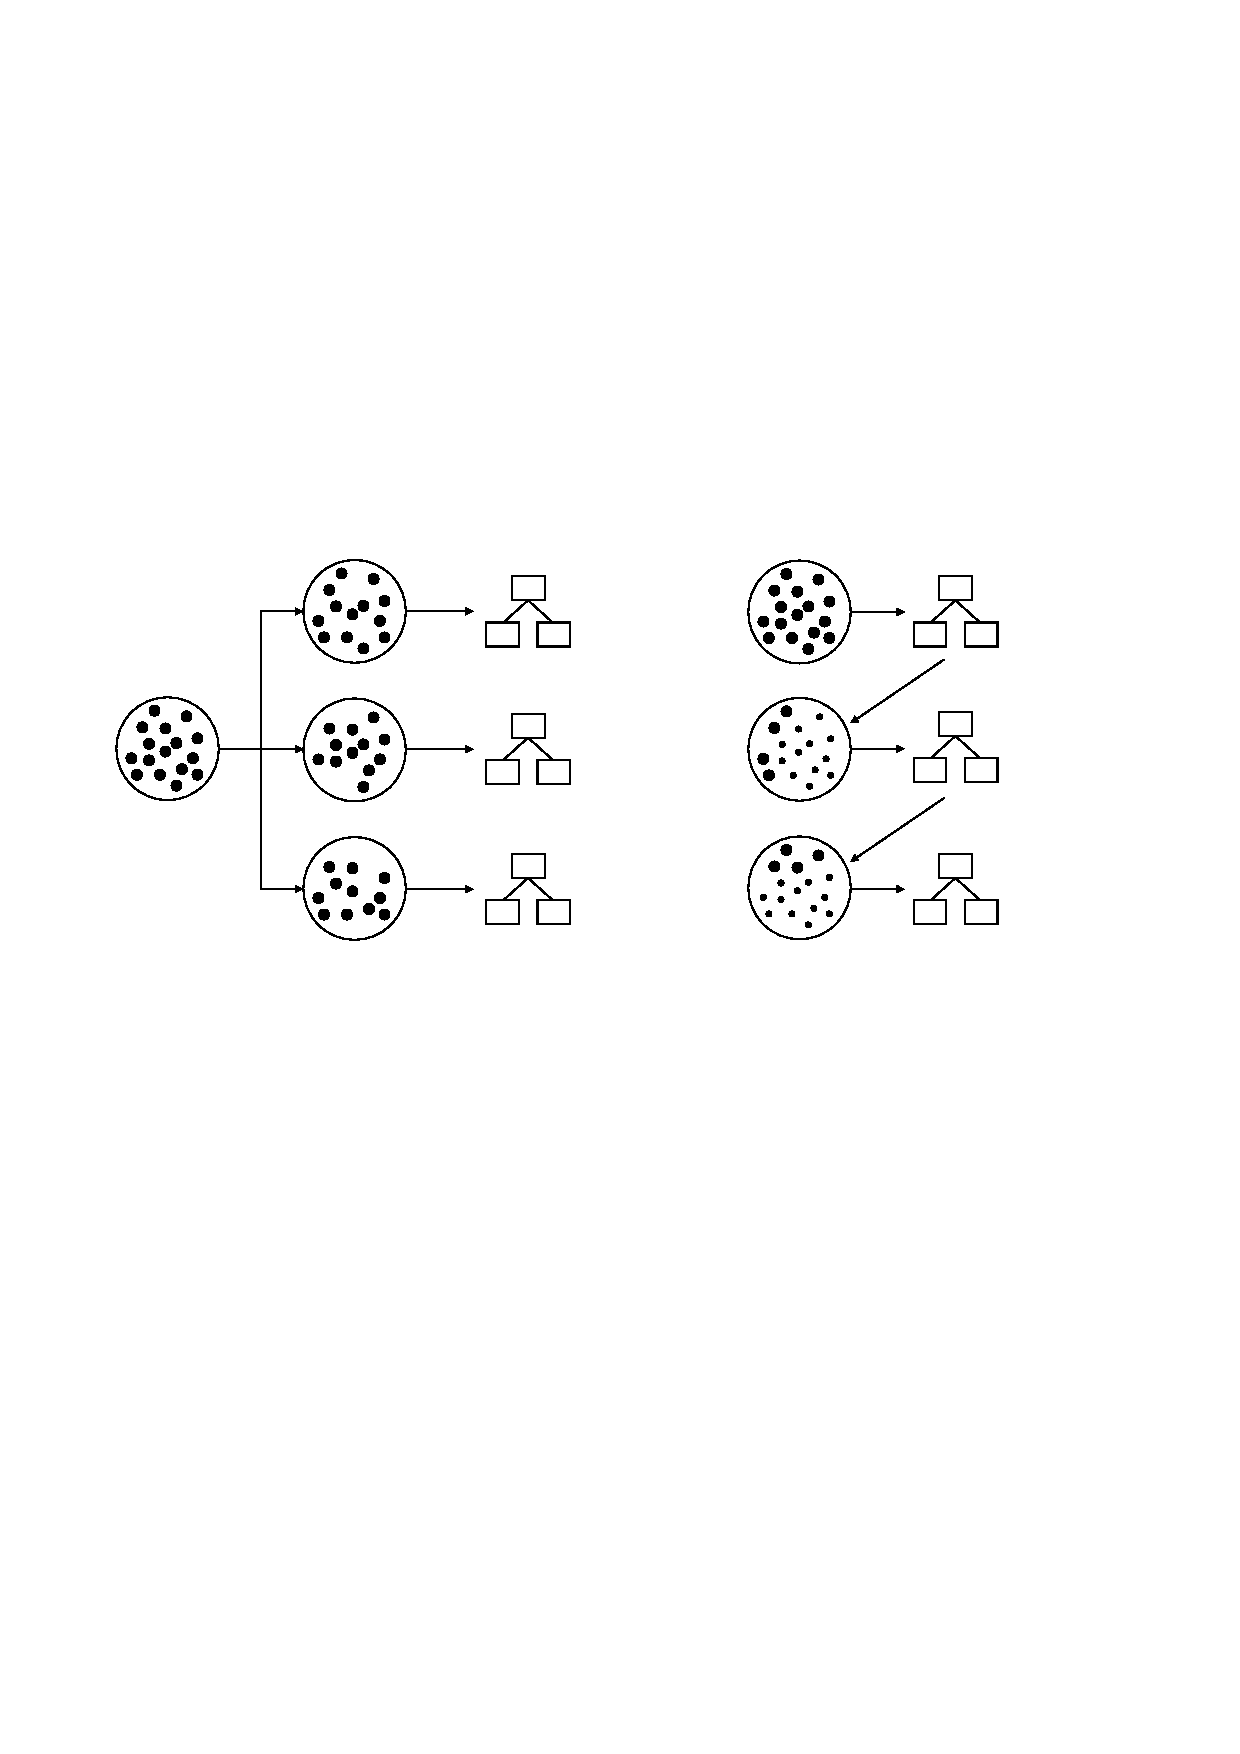
\includegraphics[width=0.8\linewidth]{figures/bagging-vs-boosting.pdf}
}
\\
\hspace{2.5cm} bagging - parallel \hspace{3cm} boosting - sequential \\
\caption{Bagging improves accuracy through ``wisdom of the crowd'', while boosting develops a sequence of models where each model specializes in prediction in the area where previous models in the sequence have failed.}
\label{fig:bagging-vs-boosting}
\end{figure}

\section{AdaBoost In a Nutshell}

Let us quickly skim through some of the concepts that are important in boosting machine learning. We use boosting both in regression and classification, and in fact, we can adapt it for any kind of supervised machine learning tasks. In this section, though, we assume we will use it for classification, and will further -- to simplify the introduction -- constrain the task to binary classification with equal class distribution.

\subsection*{Weak vs. Strong Classifiers}

Consider an error rate, $\epsilon\in[0.0,1.0]$ of a binary classifier with $y\in\{-1,1\}$ for a problem with an equal class distribution. A weak learner would produce a weak classifier that would perform only slightly better than a random classifier. That is, for an assumed problem, its error on the training set would be just slightly below $0.5$. On the other hand, in practice, we would like to develop strong classifiers with a very low error rate. Interestingly, and as a fundation for boosting, we can form a strong classifier from a set of weak classifier.

Consider a simple case of three classifiers, and let us denote them with $h^1(x)$, $h^2(x)$, and $h^3(x)$, where $x$ is a vector that describes a data instance we would like to classify. If the three classifiers are substantially different, and they make wrong predictions in disjunct areas of the data space (Fig.~\ref{fig:boosting-three-classifiers}), we can construct a simple, strong classifier as an ensemble that would join the output of the three classifiers in the following way:
\begin{equation}
H(x) = \sign(h^1(x) + h^2(x) + h^3(x))
\end{equation}
The prediction of the classifier $H(x)$, under the assumption that the areas of erroneous prediction of each of the three classifiers do not overlap. It would be great if we could construct such classifiers, but in reality, of course, the areas where classifiers get it wrong would overlap, and hence a simple procedure for their ensembling would not necessary be beneficial.

We may try to develop classifiers that are of the type from Fig.~\ref{fig:boosting-three-classifiers}, that is, where a classifier attempts to be correct in the area where a previous classifier, or a set of previous classifiers were wrong. We will do so by changing the data. We will build the first classifier, $h^1$ on the entire data set, but then try to distort the data to exaggerate on the data space where $h^1$ makes mistakes. A simple procedure we can use is through training data instance weighting: we will increase the weight of the data instances that were misclassified by $h^1$, thus instructing a new classifier $h^2$, developed on such distorted data set, to correctly classify the data instances which were misclassified by $h^1$. If we follow the idea from the previous paragraph and try to develop three different classifiers, we now can train the third one on a data set where the weights of the data instances would emphasize those $x$ where $h^1(x)\neq h^2(x)$.

Just a quick note: thus far, our classification inference algorithm never considered data instance weights. It is not difficult to change the inference algorithm to do so. For instance, in inference of trees, instead of counts of the data instances we would sum up the weights. Where changing the training algorithms to handle weights is not possible, we could address the exaggeration with oversampling of the target data instances.

\begin{figure}
\centering{
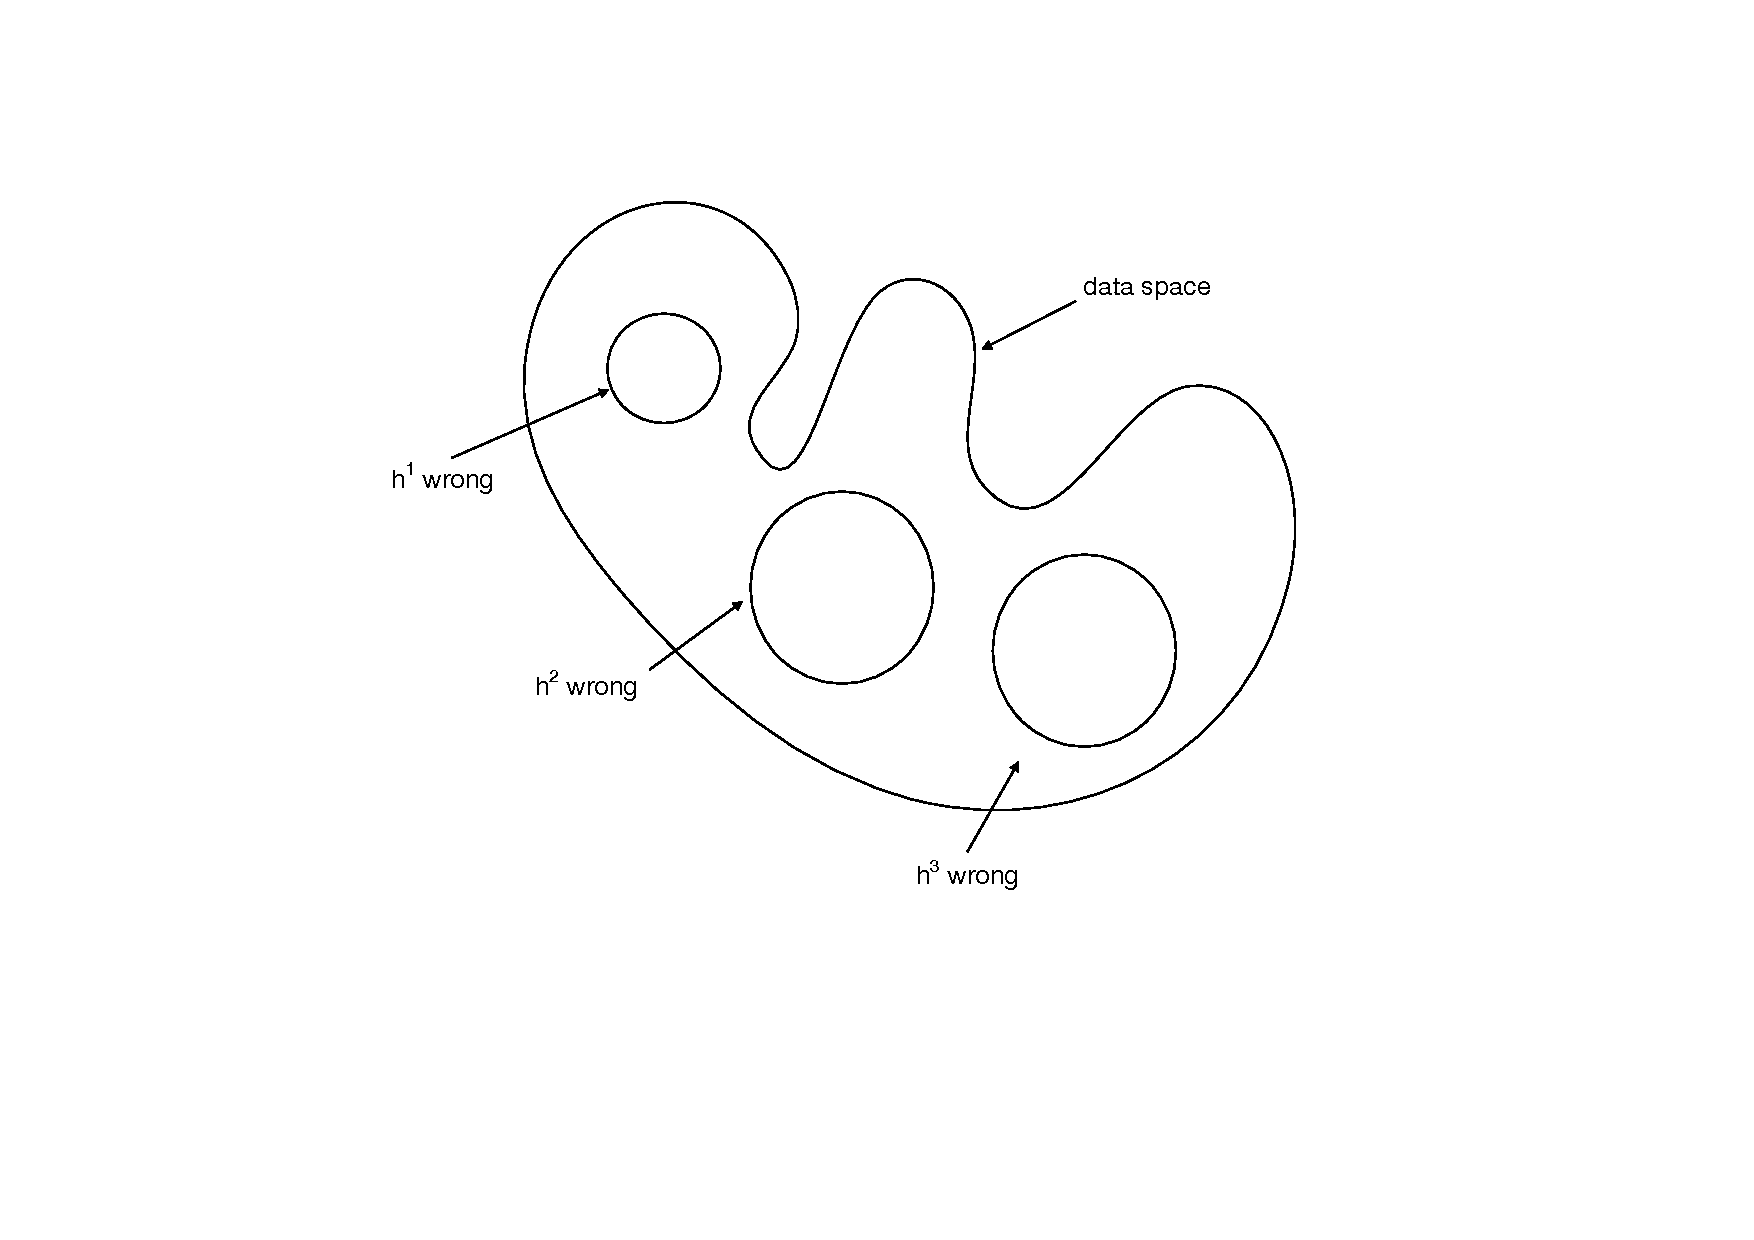
\includegraphics[width=0.5\linewidth]{figures/boosting-three-classifiers.pdf}
}
\caption{A hypothetical data space and three classifiers with disjunctive areas where their prediction is incorrect.}
\label{fig:boosting-three-classifiers}
\end{figure}

\subsection*{Hierarchy of predictors}

If constructing a classifier by ensembling the predictors works well, we could improve those predictors as well through ensembling them from another, nested set of classifiers. By doing this we would shrink the area where the predictors make mistakes, making it easier for a base set of predictors not to overlap in their misclassification zones. Note that in theory we may continue building such hierarchy to arbitrary level, whereas practically and in most cases development of one serious of predictors suffices.

\subsection*{A Weak Classifier and Initial Data Instance Weights}

We hinted about the use of weak classifiers, but have not yet introduced an algorithm to construct them. Here it is: a {\em decision tree stump}. This learning algorithm uses a decision tree inference algorithm, but limits the depth of the tree to one, that is, besides the root node there is only a next level with a set of leaves. Stumps use only one feature to decide which leave node to use for prediction. In practice, we can employ shallow trees that are deeper than one level, but for an example of a weak classifier a decision tree stumps would do as well. Also notice that while our introduction talks about classifiers, we can use trees for regression as well and hence we will also be able to develop bootstrap predictors for regression problems.

Note that we can use boosting with any kind of prediction models. But due to speed and simplicity, and since they are weak classifiers, we use shallow trees in practical implementations.

The error rate of a classifier can be expressed as:
$$\epsilon = \sum_\text{wrong}{1\over N}$$
where $N$ is the number of data instances in the training set. Initially, all instances will have equal weight and since we would like the weights to form a distribution and hence sum to $1$, the weights for each data instance $i$ for the first classifier, that is $h^1$, are:
$$w_i^1 - {1\over N}$$
Using the formulation above, we can express the error rate as a function of weights:
$$\epsilon = \sum_{\text{wrong}} w_i$$

\subsection*{Ensembling Classifiers}

A more general way to combine classifiers, rather than summing their outputs, would be to construct their weighted combination:
$$ H(x) = \sign(\alpha^1 h^1(x) + \alpha^2 h^2(x) + \ldots + \alpha^T h^T(x)) $$
where $T$ is a number of weak classifiers which we would like to ensemble. This is again different from bagging. Bagging counts on wisdom of the crowds, while here we are summing up on series of classifiers which are different in the areas of misclassification and where we will weight them according to their error. In boosting, the wisdom of the crowds becomes the wisdom of the experts that specialize in different area of the data space.

The overall procedure to construct our ensemble is then as shown in Table~\ref{t:bootstrap-algorithm}.

\begin{table}
\caption{An overall structure of a bootstrap learner}
\begin{tabbing}
xxxx \= xxxx \= xxxx \kill
$t\leftarrow 0$ \\
$w_i^t\leftarrow {1\over N}$ \\
{\bf while} $t\leq T$ \\
\> $t\leftarrow t+1$ \\
\> {\bf pick} $h^t$ that minimizes $\epsilon^t$ \\
\> {\bf pick} $\alpha^t$ \\
\> {\bf calculate} $w^{t+1}$
\end{tabbing}
\label{t:bootstrap-algorithm}
\end{table}

Suppose that we define the weights as:
$$w_i^{t+1}={w_i^t\over z} \exp\left(-\alpha^t h^t(x_i)y_i\right)$$
where $z$ is a normalizing factor so that the weights form a distribution and they sum to 1. The equation above comes from mathematical convenience, but we will show that while initially proposed for boosting, they have a more intuitive and simpler interpretation. Notice that where the prediction $h^t(x_i)$ and the true class $y_i$ agree, and assuming that the factors $\alpha$ are positive, the future weight $w_i^{t+1}$ of the instance $i$ is lowered. When prediction and the true class do not agree, the value of the future weight $w_i^{t+1}$ is raised.

We would like to minimize the error for the ensemble. It turns out that to do this~\citep{FreundSchapire1997} we need to set the weight of the classifier according to the following:
\begin{align}
\alpha^t & ={1\over 2}\ln{1-\epsilon^t \over \epsilon^t} \label{eq-freundschapire}\\
& = \ln{\sqrt{1-\epsilon^t \over \epsilon^t}}
\end{align}

If we combine this expression with the update for the data instance weights, and note that the product $h^t(x_i)y_i$ equals $1$ for correct classification and $-1$ for misclassification, than we obtain
$$w_i^{t+1} = {w_i^t \over z} \times
\begin{cases}
\sqrt{\epsilon^t \over 1-\epsilon^t }, & \text{if correct} \\
\sqrt{1-\epsilon^t \over \epsilon^t}, & \text{if wrong}.
\end{cases}
$$
The weights have to add up to 1, thus we need to set the normalization factor to
$$
z = {\epsilon^t \over 1-\epsilon^t} \sum_\text{correct} w_i^t + {1-\epsilon^t \over \epsilon^t}\sum_\text{wrong} w_i^t
$$
Notice, however, that the sum of the weights of the missclassified items is the error rate, that is, $\sum_\text{wrong} w_i^t=\epsilon^t$. Similarly, the sum of the weight over correct classifications is one minus the error rate, that is, $\sum_\text{correct} w_i^t=1-\epsilon^t$. Hence,
$$
z = 2\sqrt{\epsilon^t (1-\epsilon^t)}
$$
Combining the expression for weight update and normalization, we obtain:
$$w_i^{t+1} = {w_i^t \over 2} \times
\begin{cases}
\sqrt{1\over 1-\epsilon^t }, & \text{if correct} \\
\sqrt{1\over \epsilon^t}, & \text{if wrong}.
\end{cases}
$$
Now, if we add the weights for the correct classifications, we get
\begin{align*}
{1\over 2}{1\over 1-\epsilon^t}\sum_\text{correct} w^t & = {1\over 2}{1\over 1-\epsilon^t} (1-\epsilon^t)\\
& = {1\over 2}
\end{align*}
Similar is true for missclassifications,
\begin{align*}
{1\over 2}{1\over \epsilon^t}\sum_\text{wrong} w^t & = {1\over 2}{1\over \epsilon^t} \epsilon^t\\
& = {1\over 2}
\end{align*}

In other words, the boosting algorithm that we have described distrubutes the same amount of weights to correct and incorrect classification. If incorrect classifications will be in minority, which we hope they will, the misclassified examples will carry higher weights for the next instance of the training algorithm in the sequence. The procedure described here is called AdaBoost for adaptive boosting and was introduced in ~\citep{FreundSchapire1997}. Interestingly, while the math for Eq.\ref{eq-freundschapire} was worked out in the original publication, the interpretation with notion that the weights for both misclassification and classification sum to one half, which does in a way simplify the update as well, was not noticed at the time.

% \section{AdaBoost}

% AdaBoost, as described in the previous section, is an example of a boosting machine learning procedure that sequentially applies the weak classification algorithm to repeatedly modified version of the training data by increasing the weights of the misclassified data instances. The procedure dramatically increases the performance of weak learners, which is shown in often exponential decrease of the error rate on the test set with increasing number of classifiers in the sequence. We here explore why is this so, what loss function are we optimizing and the review other algorithms in this class.

% Let us start with the decision rule, or the output of the AdaBoost with $M$ predictors:
% \begin{equation}
% H(x)=\sign\left( \sum_{m=1}^M \alpha^m h^m(x)) \right) 
% \end{equation}


\printbibliography[heading=subbibliography]
\end{refsection}
\begin{refsection}
\chapter{Artificial Neural Networks}

\begin{summary}
Neural networks combine incredibly simple computational units to solve possibly the hardest problem in machine learning: discovery of feature interactions. Initially inspired by architectures of neurons and brains, they model these very loosely but equally build their power on the number of connections and parallel processing. In this lecture, we provide an elementary introduction to artificial neural networks. We focus on motivation, describe inspirations from biology, and delve into perceptron and its failures. Next, we introduce the artificial neuron and the combinations of neurons within the standard feed-forward neural network. We show how to compute the gradient of the cost function with respect to the parameters of the model. Computation of the gradients uses chain rules and led to the algorithm for weight updates called backpropagation. We finish with some ideas on optimization and avoidance of overfitting, and mention, but do not delve into, other types of neural networks.
\end{summary}

The computational motivation for introduction of neural networks are to learn {\em hard} concepts. For instance, consider a concept depicted in Fig.~\ref{fig:hard-concept}: the classification rule that separates the classes needs to model interaction between the two features. Assuming the other features or combinations are not as informative as a combination from Fig.~\ref{fig:hard-concept}, and supposing that the training data set that contains $1.000$ features, one would need to search among $999.000$ feature pairs to find the informative pair. If a concept involves a feature triplet, the search size is larger and contains $332.334.000$ triplets. Addressing such problem directly, through exhaustive search, is computationally not feasible.\footnote{Actually, and depending on a data set, it is also statistically not feasible, but we will leave this problem aside.}

\begin{figure}
\centering{
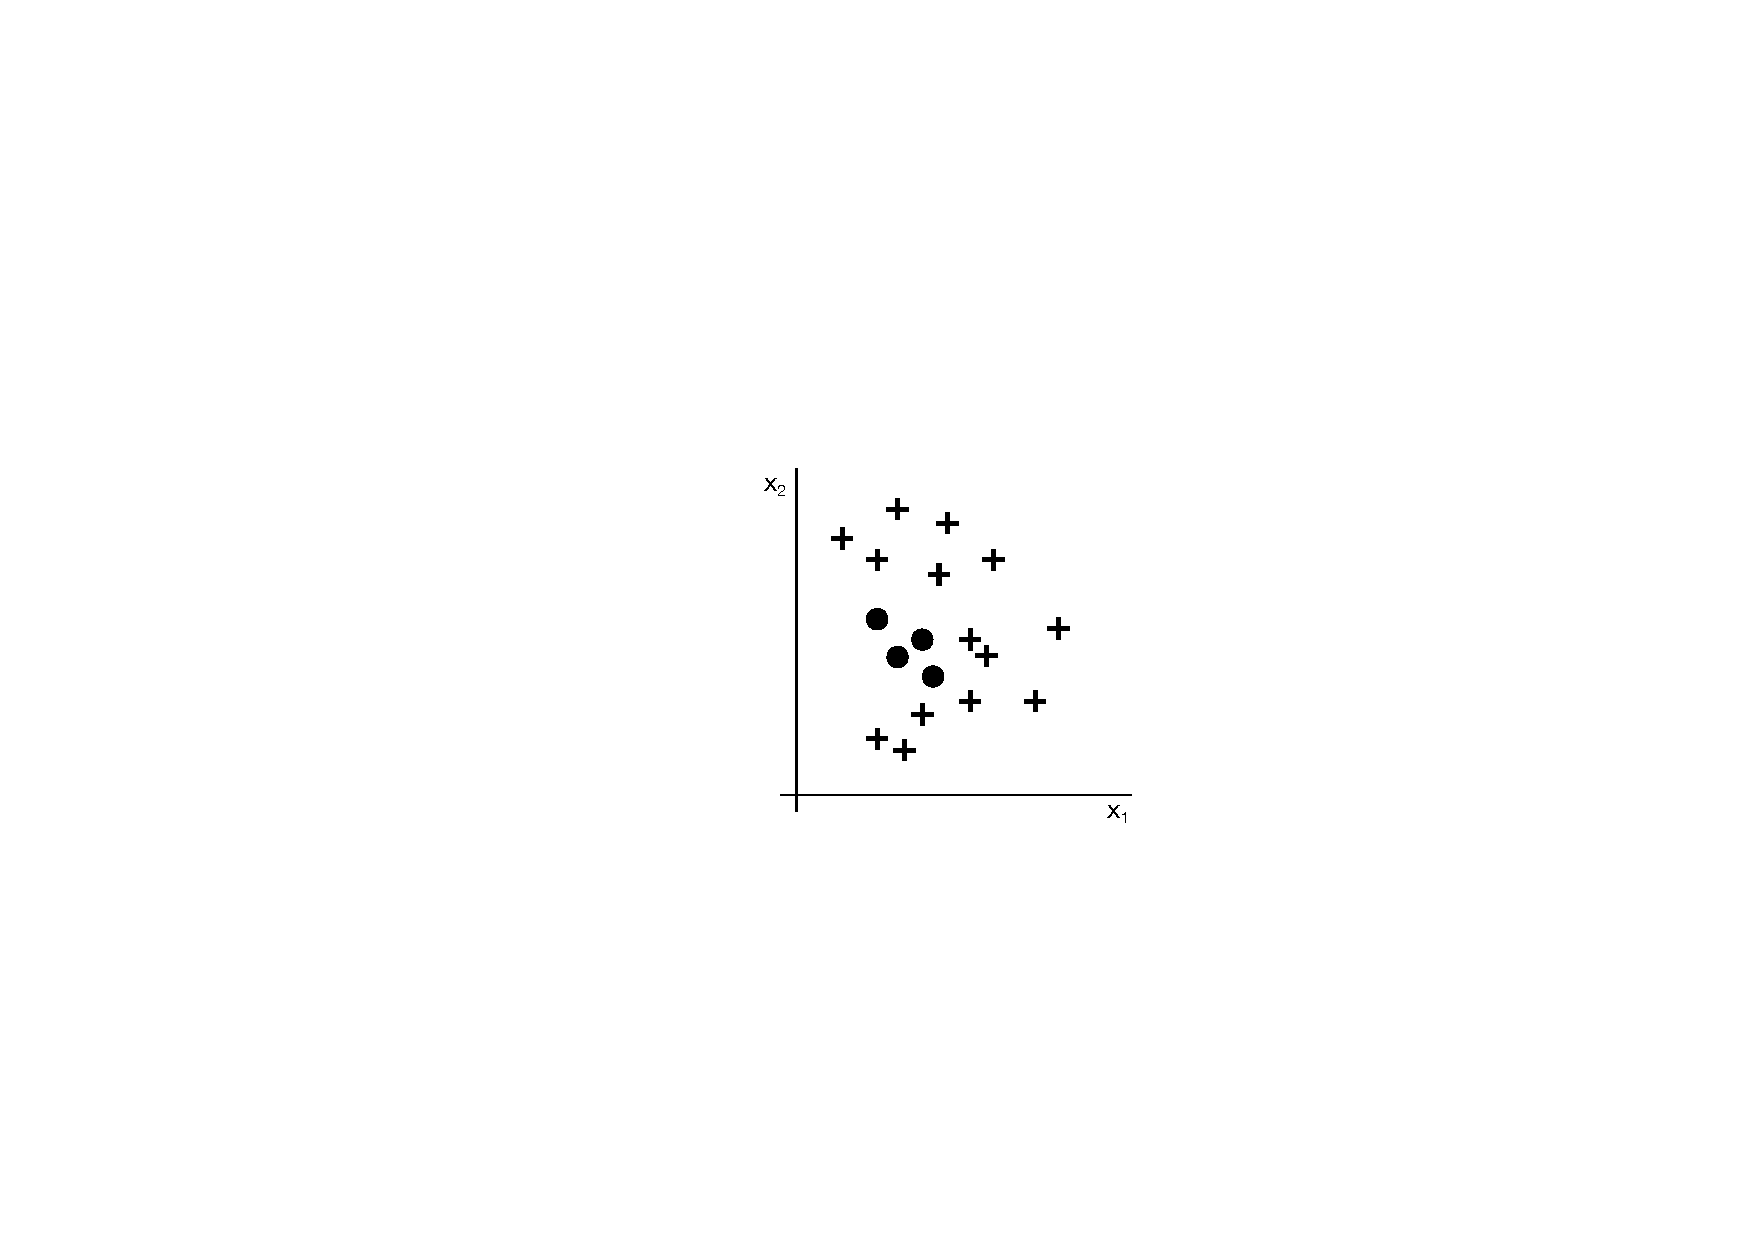
\includegraphics[width=0.3\linewidth]{figures/ann-hard-concept.pdf}
}
\caption{An example of a hard classification concept, where the classifier would need to recognize the interaction between two features, $x_1$ and $x_2$. Concepts like these are especially hard to model in the presence of many other features, which can be to a degree related to the class.}
\label{fig:hard-concept}
\end{figure}


A possible alternative to exhaustive search of feature interactions are models that incorporate feature interaction, and that can possibly model any kind of interaction between any of the features. The problem we are facing is of course the data. Such models need substantial, if not huge amount of data for training to avoid overfitting. But if data is available -- and sometimes it is -- then we better define the model that we can use in such cases. Notice that we are moving into direction where such models may be hard to explain, but this also is an issue we will deal with later, in our next chapter.


\section{Motivation from biology}

We start with disclaimer: artificial neural networks are very simplistic model of a brain, or any biological neural network. Biology is by orders of magnitude more complex: an axon, that is considered in artificial networks as a wire, has been studies in numerous projects and its structure and physiology has been reported in books of thousands of pages. With this warning, though, consider a realistic model of a neural cell in Fig.~\ref{fig:neural-cell}. Neural cell emits electric signals through the axon, but only when the potential in the cell body reaches a certain level, called {\em action potential}. The electrical potential of the body is a sum of potentials in the dendrites, and and this in turn depend on potential evoked from connected cells. Connections are established through synapses, which chemically transmit the electrical signal from the axon tips (inputs) to the dendrites. Neural cells thus, in a very simplified way, sum up the input signals and fire when the sum reaches specific threshold, emitting the signal through the axon and establishing a network with connected cells.

\begin{figure}
\centering{
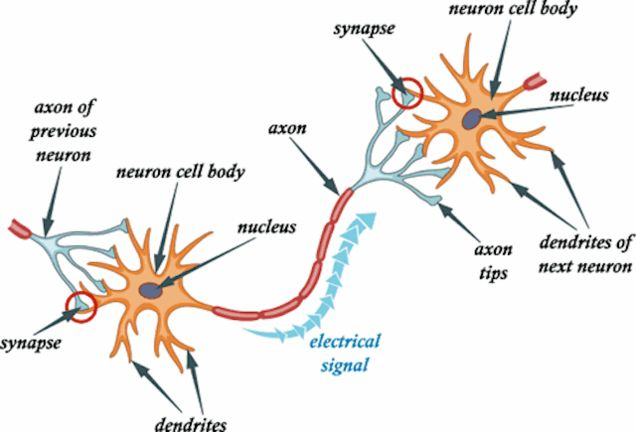
\includegraphics[width=0.8\linewidth]{figures/ann-neural-cell.jpg}
}
\caption{The structure of a neural cell, showing means of communication between two connected cells.}
\label{fig:neural-cell}
\end{figure}


Human brain contains $8\times 10^{10}$ neurons, where, on average, each neuron is connected to $10.000$ other neurons. The resulting network is huge and contains $10^{15}$, that is, $1.000$ trillion connections. 

Synapses adapt, adjusting the quantity of required transmitters and available receptors, thus implementing one of the mechanisms for plasticity of the brain and learning. Synapses, on the other hand, implement chemical transmission of the signals and are thus slow, but they are many and function in parallel.

The brain is modular. Different regions perform different functions. Experimentally this was observed in patients where local damages had specific effects. But the plasticity was observed as well: regions of brains can take over a specific function after the brain region originally carrying out this function was damaged. Damage in one region can therefore be alleviated through specialization of another region.

The idea of the network of neurons, neurons summing up the input signals, adaptivity of synapses which can weight the input, and a activation function implemented by a body of a neural cell are all concepts that are modeled by artificial neural networks. Brain plasticity and redundancy are modeled as well, and specifically addressed in larger, deeper neural networks.

\section{Idealized neuron}

Idealized neuron is a model of a neuronal cell with complicated details removed (Fig.~\ref{fig:idealized-neuron}). It performs simple mathematics, resorts to basic principles, and is wrong since the communication is not binary. The simplest model sums-up the inputs through a weighted sum, where $w_i$ is a weight for $i$-th input:
\begin{equation}
z = b + \sum_i x_i w_i,
\end{equation}
and the output of the {\em linear neuron} is
\begin{equation}
\hat{y} = z
\end{equation}

\begin{figure}
\centering{
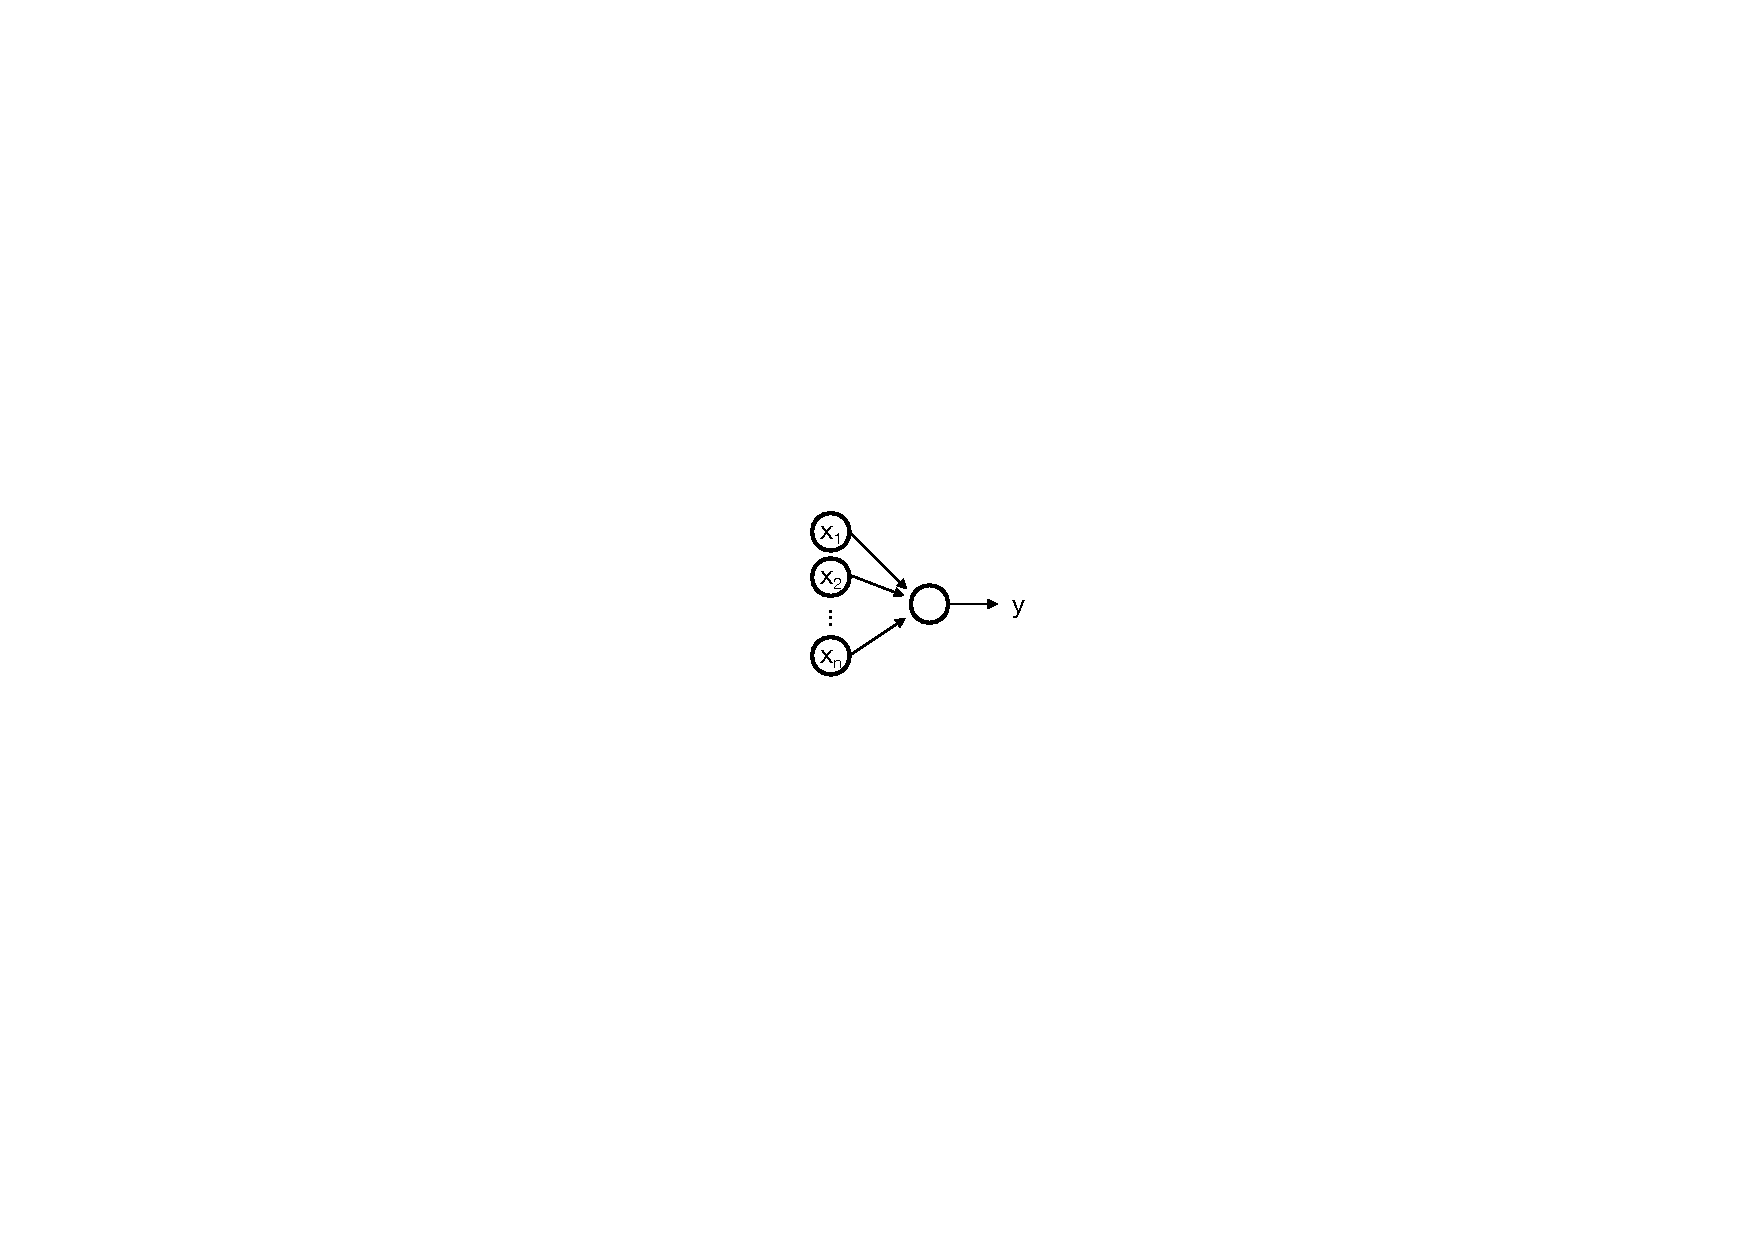
\includegraphics[width=0.3\linewidth]{figures/idealized-neuron.pdf}
}
\caption{An idealized neuron with $x_i$ representing its inputs and $y$ an output variable.}
\label{fig:neural-cell}
\end{figure}

Other types of neurons incorporate other {\em activation functions}, that is, functions that take a weighted sum of the inputs to compute the output of a neuron. Popular examples include {\em binary threshold neuron},
\begin{equation}
\hat{y} = 
\begin{cases}
1 & \text{if } z\geq 0 \\
0 & \text{else}
\end{cases}
\end{equation}
{\em rectified linear neuron}, or RELU,
\begin{equation}
\hat{y} = 
\begin{cases}
z & \text{if } z\geq 0 \\
0 & \text{else}
\end{cases}
\end{equation}
and {\em sigmoid neurons},
\begin{equation}
\hat{y}={1\over 1+e^{-z}}
\end{equation}
Notice that a sigmoid neuron looks very much like one of the classification models we have already studied. Which one, and what are the differences, if any?

\section{Perceptrons}

Training with a single linear neuron, that is, a neuron implementing $z=w^\tr x$ and a related classifier, 
\begin{equation}
\hat{y} = h(z) =
\begin{cases}
1 & \text{if } z\geq 0 \\
-1 & \text{else}
\end{cases}
\end{equation}
was popular in 1960s under the name perceptron. The perceptrons (Fig.~\ref{fig:perceptron-learning}, algorithm in Table~\ref{t:perceptron}) were proposed by Frank Rosenblatt, one of the pioneers of artificial intelligence, and were wrongly presented as a very powerful tool. In really, learning with perceptrons was very weak, could not handle noise, but is still historically interesting. 

\begin{table}[htbp]
\caption{Perceptron's learning procedure}
\begin{tabbing}
xxxx \= xxxx \= xxxx \= xxxx \kill
initialize $w$ \\
{\bf repeat} \\
\> choose $(x, y)$ from the training set \\
\> {\bf if} $h(z) \neq y$ \\
\> \> {\bf if} $h(z)=-1$ \\
\> \> \> $w\leftarrow w+x$ \\
\> \> {\bf else} \\
\> \> \> $w\leftarrow w-x$ \\
\end{tabbing}
\label{t:perceptron}
\end{table}

\begin{figure}[htbp]
\centering{
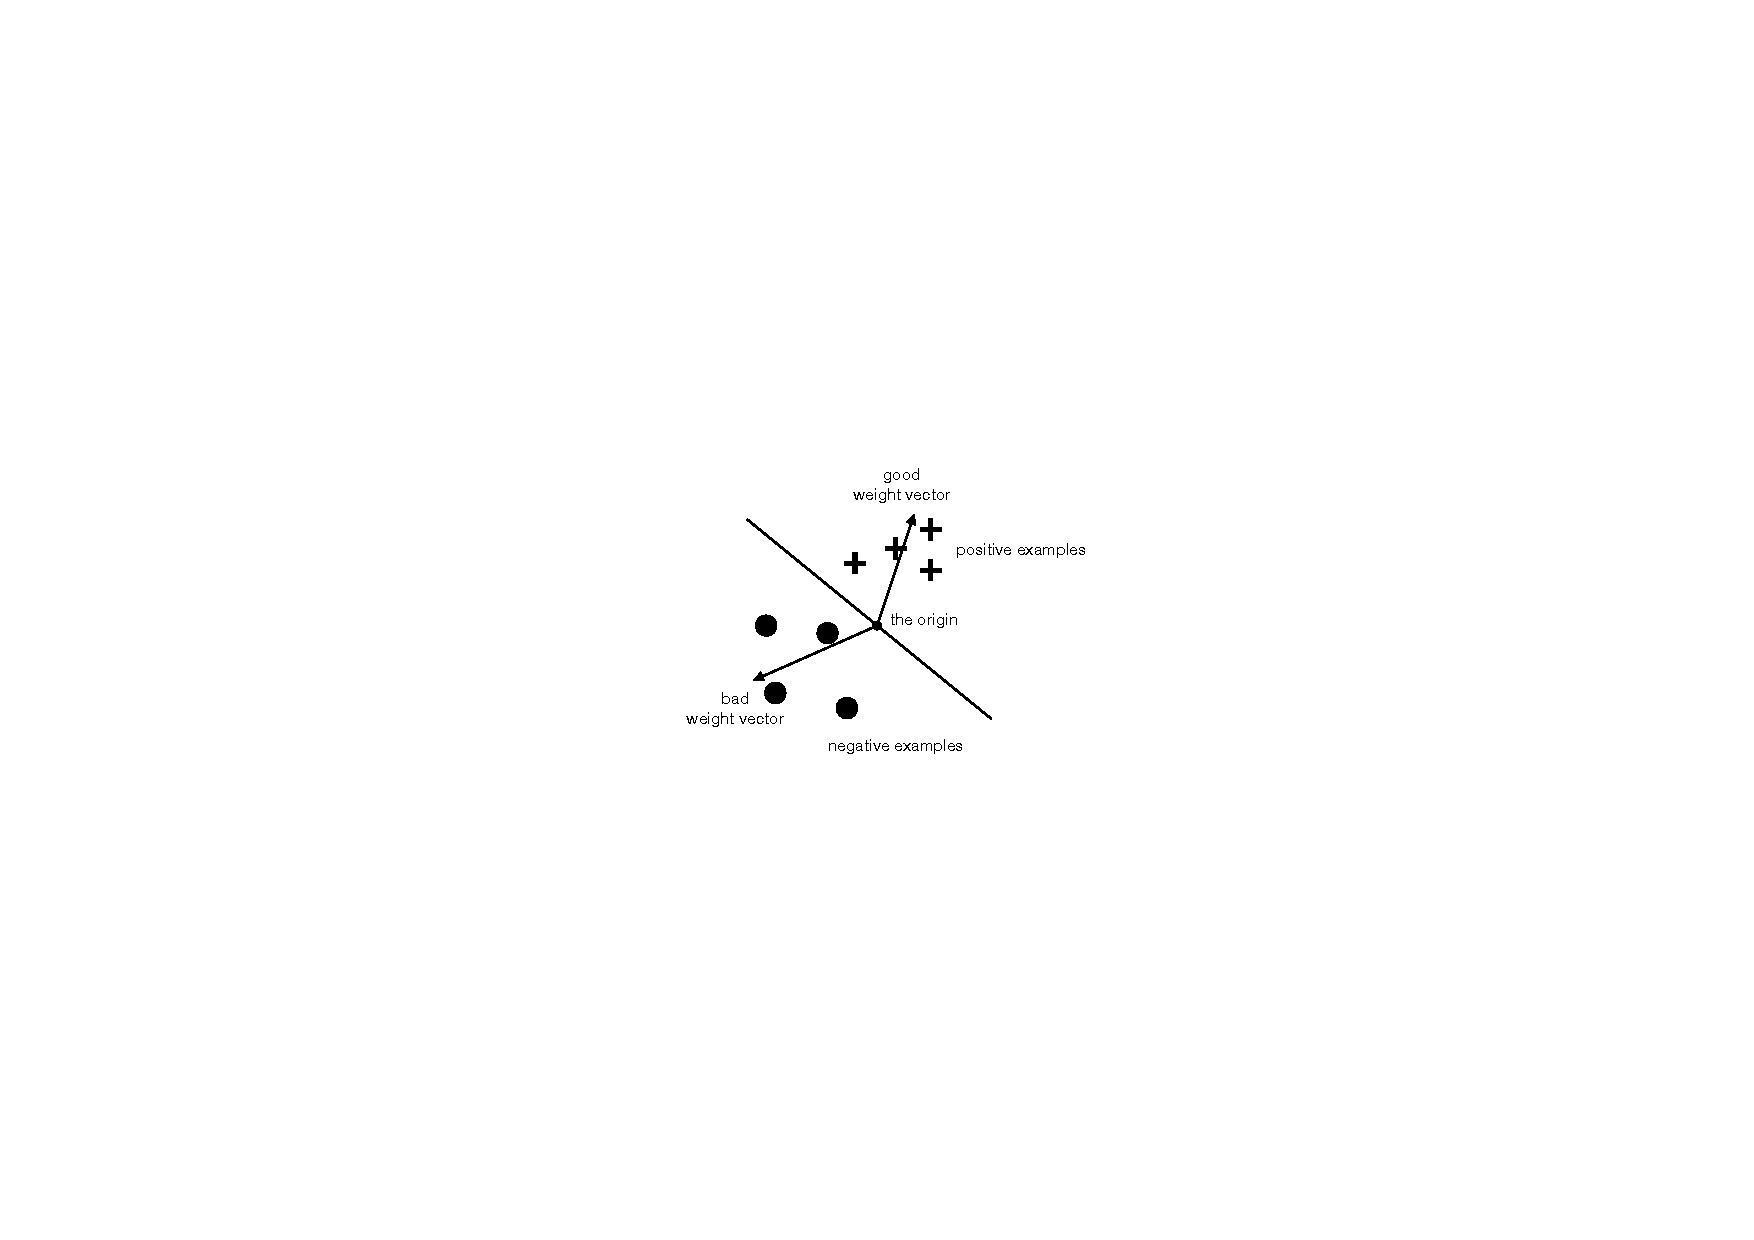
\includegraphics[width=0.3\linewidth]{figures/perceptron-learning.pdf}
}
\caption{Several concepts in perceptron learning.}
\label{fig:perceptron-learning}
\end{figure}

Notice that the perceptron training (Table~\ref{t:perceptron}) actually implements a stochastic gradient descent with a batch size of one and a learning rate of one. The training would succeed in cases where the classes are linearly separable, but fail otherwise. In linearly separable cases there would be infinitely many solutions where perceptron training would converge to a particular one. The process would fail under any interaction between input variables, where a typical example would be that of XOR. Obviously, there, we would need hierarchy of concepts and a nested perceptrons to model interactions.

\section{Artificial neural networks}

Artificial neural network is a network of artificial neurons. Output of one neuron is fed into inputs of a set of neurons. While there is no limitation on the structure of the network, the typical network starts with a layer of input features, continues with a layer of neurons, and then with the next layers, where each layer is fully connected. That is, a neuron at layer $L$ receives inputs from all neuron at previous level, level $L-1$. The last layer is special, and set according to the problem at hand. For instance, for regression, the last layer may include only one neuron, whose activation models variable $y$. For classification, the last layer may have as many neurons as there are class values, where each activation reports on a class probability. We refer to all layers between an input layer and an output layer as {\em hidden} layers.

Just like with other machine learning techniques, we have to set a cost function, and define a procedure to optimize the weights for each of the neuron accordingly. This procedure is known as {\em back-propagation}, and actually implements a gradient descent. We develop the mathematics for it in the next section.

\section{Back-propagation algorithm}

We start with some conventions. We assume that all units of the neural network can take value between 0 and 1. We refer to this value as {\em activation} and will denote it with $a$. In the previous text, when introducing a single neuron, we have denoted it with $\hat{y}$, which we will now reserve for the output of the entire network. We will also assume that the output of the neural network corresponds either to the value of regression problem, or to class probabilities, where of form of softmax regression is used to guarantee that the class probabilities sum to one.

To introduce the notation, consider a simple neural network with one input feature $x$ and one output $\hat{y}$, and one neuron in each of the two hidden layers (Fig.~\ref{fig:simple-network}).

\begin{figure}[htbp]
\centering{
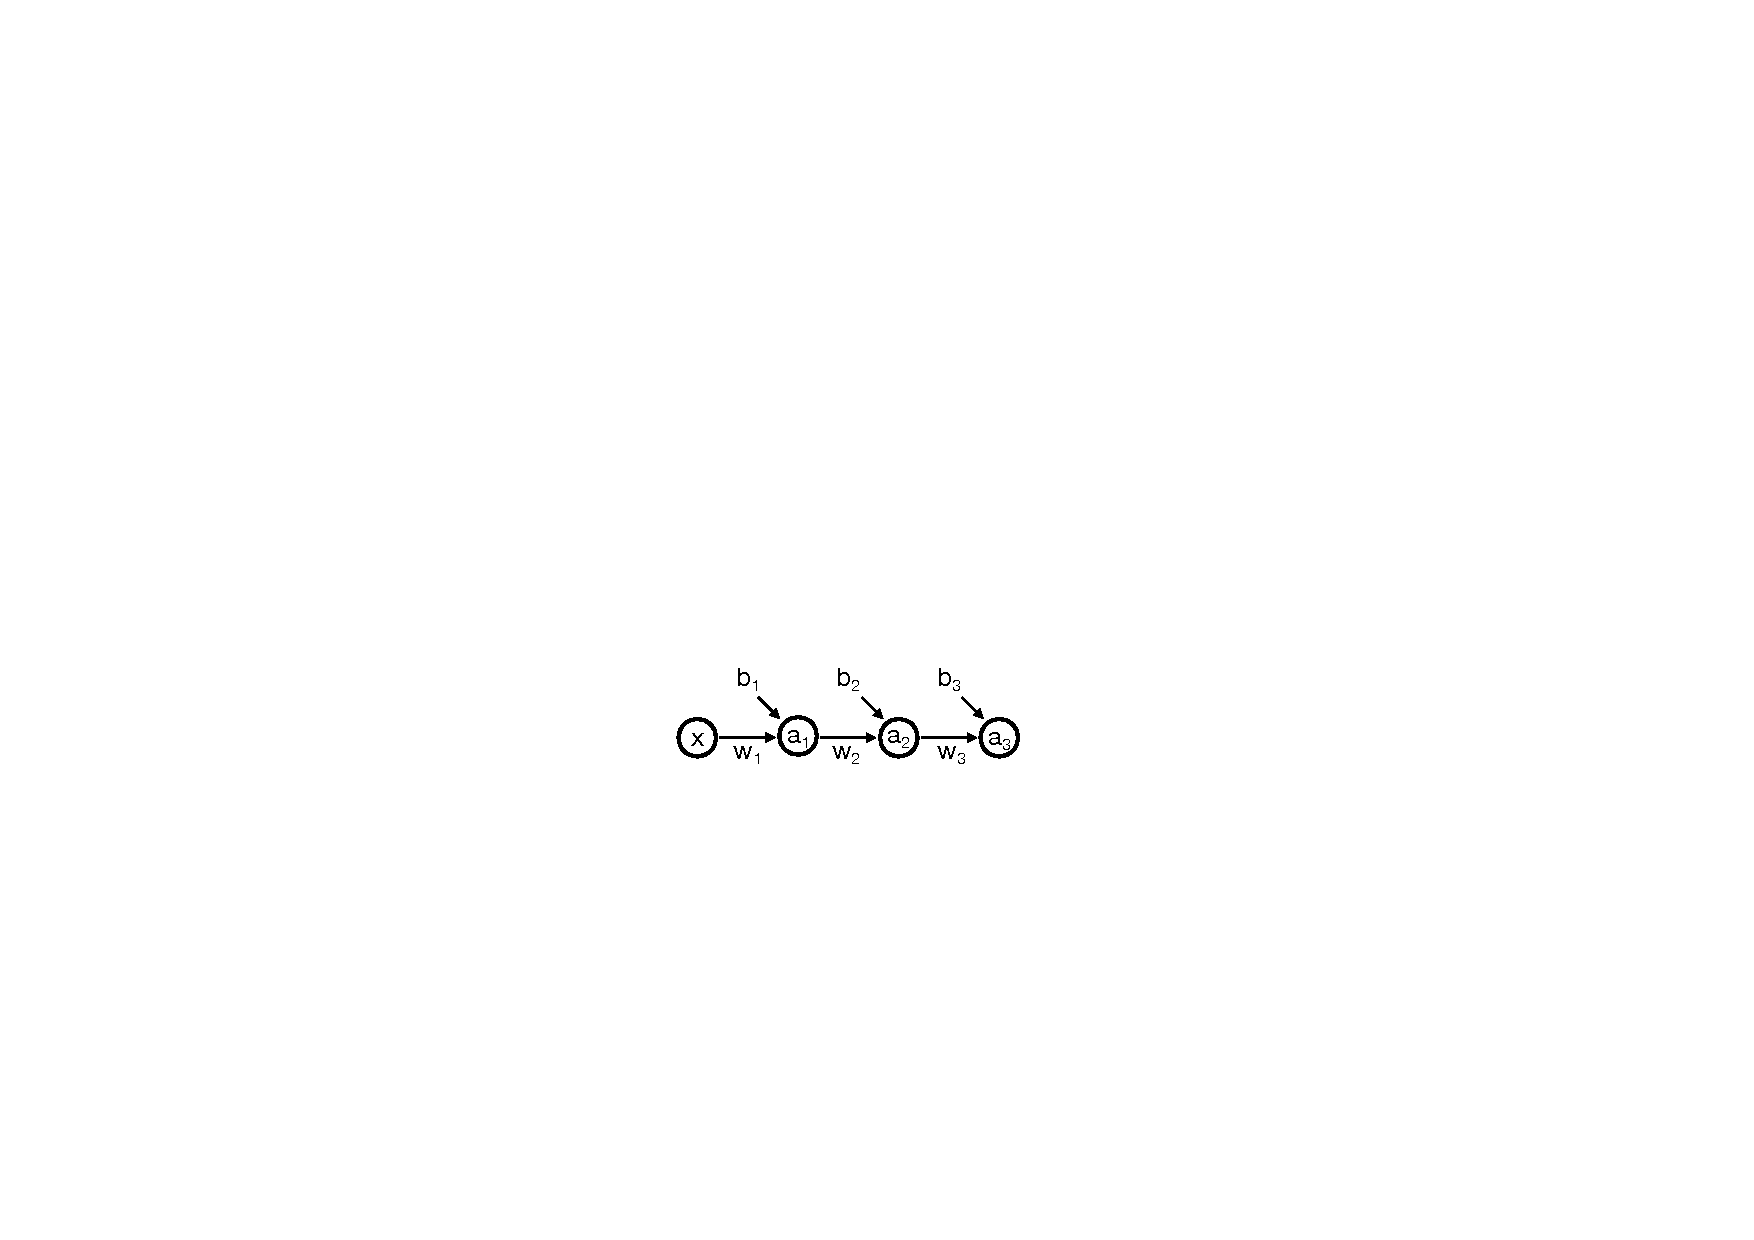
\includegraphics[width=0.5\linewidth]{figures/simple-network.pdf}
}
\caption{An example of a network with a single input and output and one neuron per layer.}
\label{fig:simple-network}
\end{figure}

Let us, for simplicity, assume we are dealing with only one example in the training set, and define a cost function as a squared error:
\begin{equation}
J(w_1, b_1, \ldots, w_3, b_3)=(a_3-y)^2
\end{equation}
Until now, we have used the indices to denote the weights $w$, the offsets $b$ and activation at each layer. Later, when dealing with more than one neuron at each layer, a notation which denotes the layer number will come handy. Apart from the layer with the input value, our simple network from Fig.~\ref{simple-network} has three layers, $L=3$. The activation $a_3$ belongs to the third layer and we will alternatively denote it with $a^{(L)}$. Similarly, $a^{(L-1)}$ will denote $a_2$. Same goes with other parameters and activation values. We can thus write that the weighted sum of inputs for neuron at layer $L$ is equal to
\begin{equation}
z^{(L)}=w^{(L)} a^{(L-1)}+b^{(L)},
\end{equation}
the activation of that neuron is
\begin{equation}
a^{(L)}=\sigma(z^{(L)}),
\end{equation}
and the cost function
\begin{equation}
J(w_1, b_1, \ldots, w_3, b_3)=(a^{(L)}-y)^2
\end{equation}
While we can use any activation function here, we will sigmoid activation function for convenience.

To implement gradient descent, we need to find how does a cost function $J$ depend on the values of the parameters of the neural network. For instance, how does $J$ depend on the weight $w_3$, that is, the weight $w^{(L)}$? We can use a chain rule to compute the partial derivate, and while doing so, it helps us to examine the dependencies as depicted in Fig.~\ref{fig:dependency-tree}:
\begin{align}
\pd{J}{w^{(L)}} & = \pd{z^{(L)}}{w^{(L)}} \times \pd{a^{(L)}}{z^{(L)}} \times \pd{J}{a^{(L)}}\\
& = a^{(L-1)} \times \sigma(z)(1-sigma(z)) \times 2(a^{(L)}-y).
\end{align}
We can interpret the terms in this equation as $a^{(L-1)}$ denoting the power (or the weight) of the precious layer, $\sigma(z)(1-sigma(z))$ denoting a derivative of an activation function, and term $2(a^{(L)})-y)$ as the error of the prediction.

\begin{figure}[htbp]
\centering{
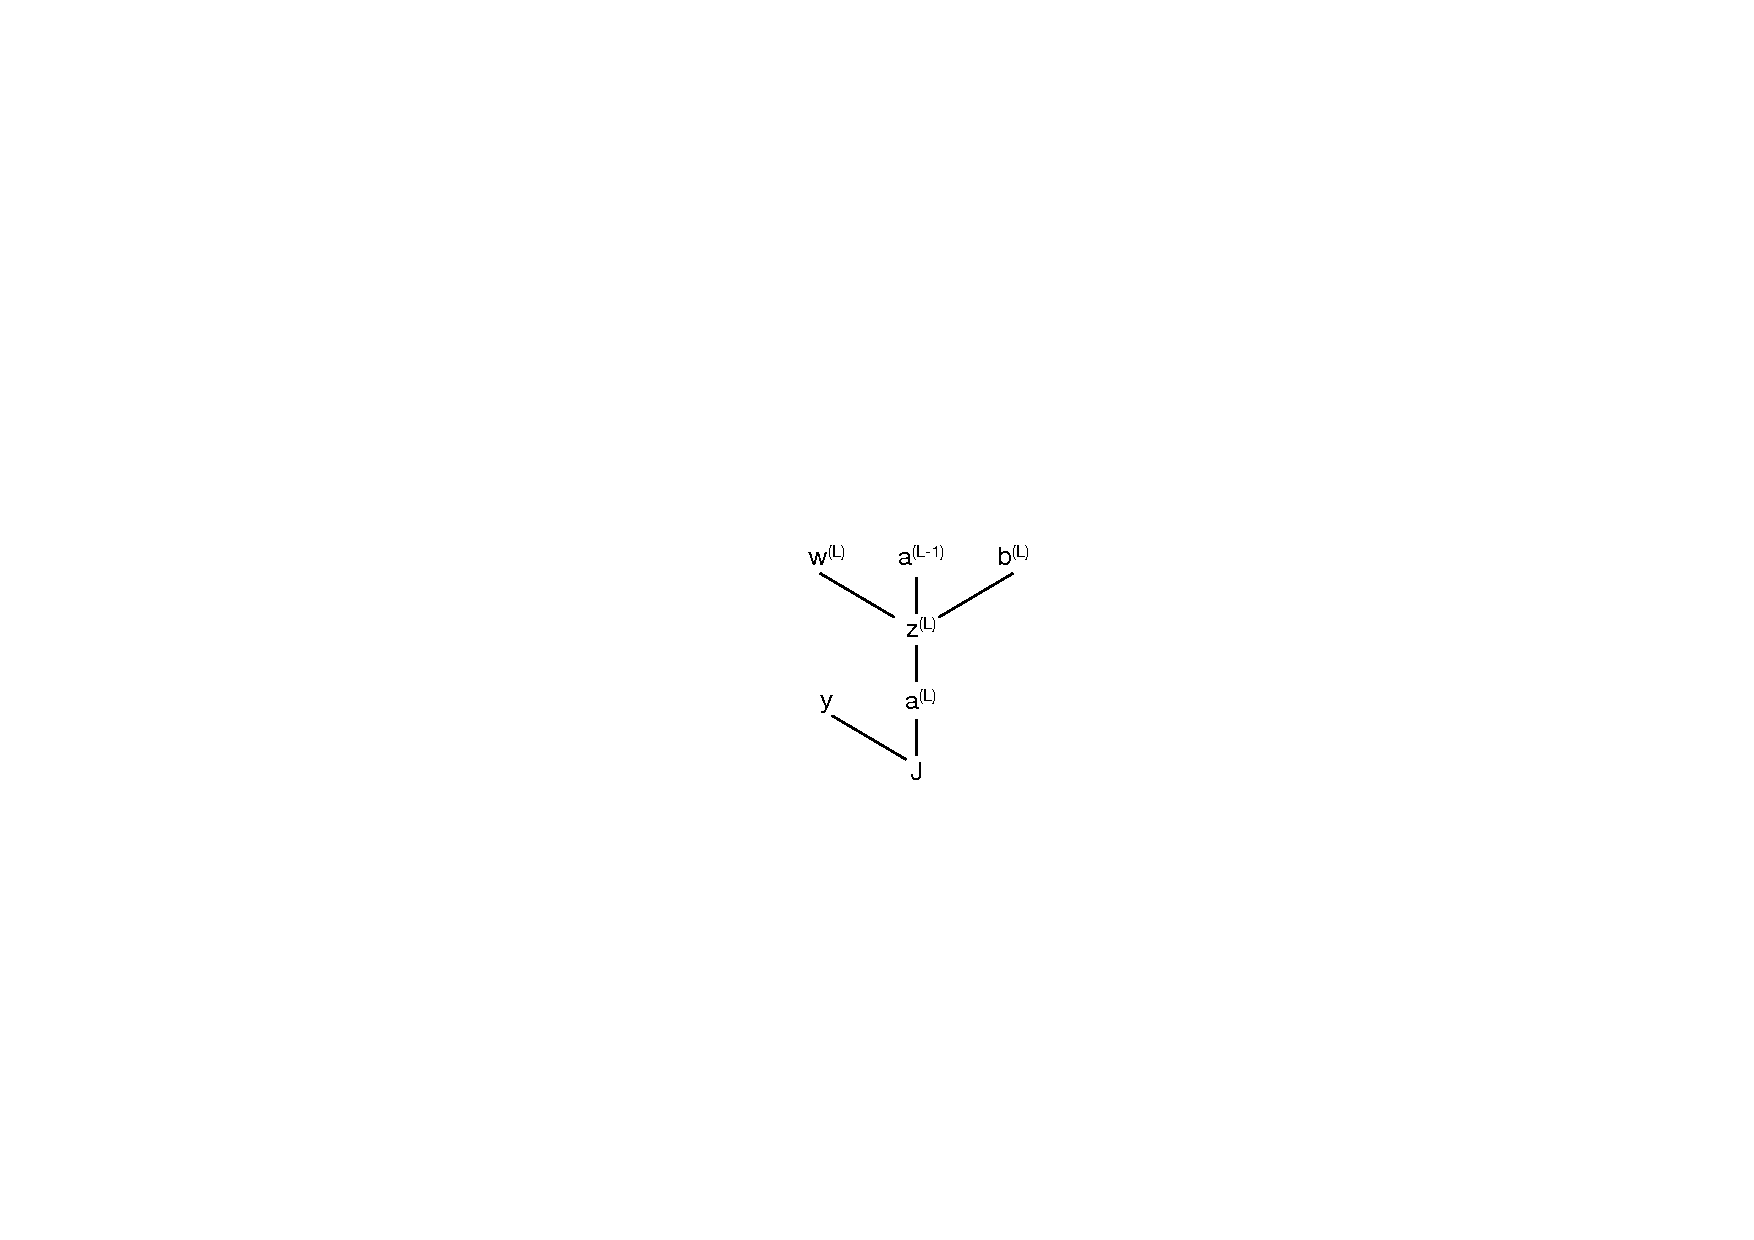
\includegraphics[width=0.3\linewidth]{figures/ann-dependency-tree.pdf}
}
\caption{Dependency tree of the cost function $J$ on some of the parameters from the neural network from Fig.~\ref{fig:simple-network}.}
\label{fig:dependency-tree}
\end{figure}

Above we have assumed we are dealing with only one training example. To generalize the above assertions for a set of training instances, we first need to modify the definition of the cost function, which now becomes:
\begin{equation}
J = \sum_{j=0}^N\left(a_j^{(L)}-y_j\right)^2
\end{equation}
Notice that the only change when computing partial derivative of $J$ according to $w^{(L)}$ is in computation of third term, $\pd{J}{a^{(L)}}$, which now becomes a sum of partial derivates.

\begin{figure}[htbp]
\centering{
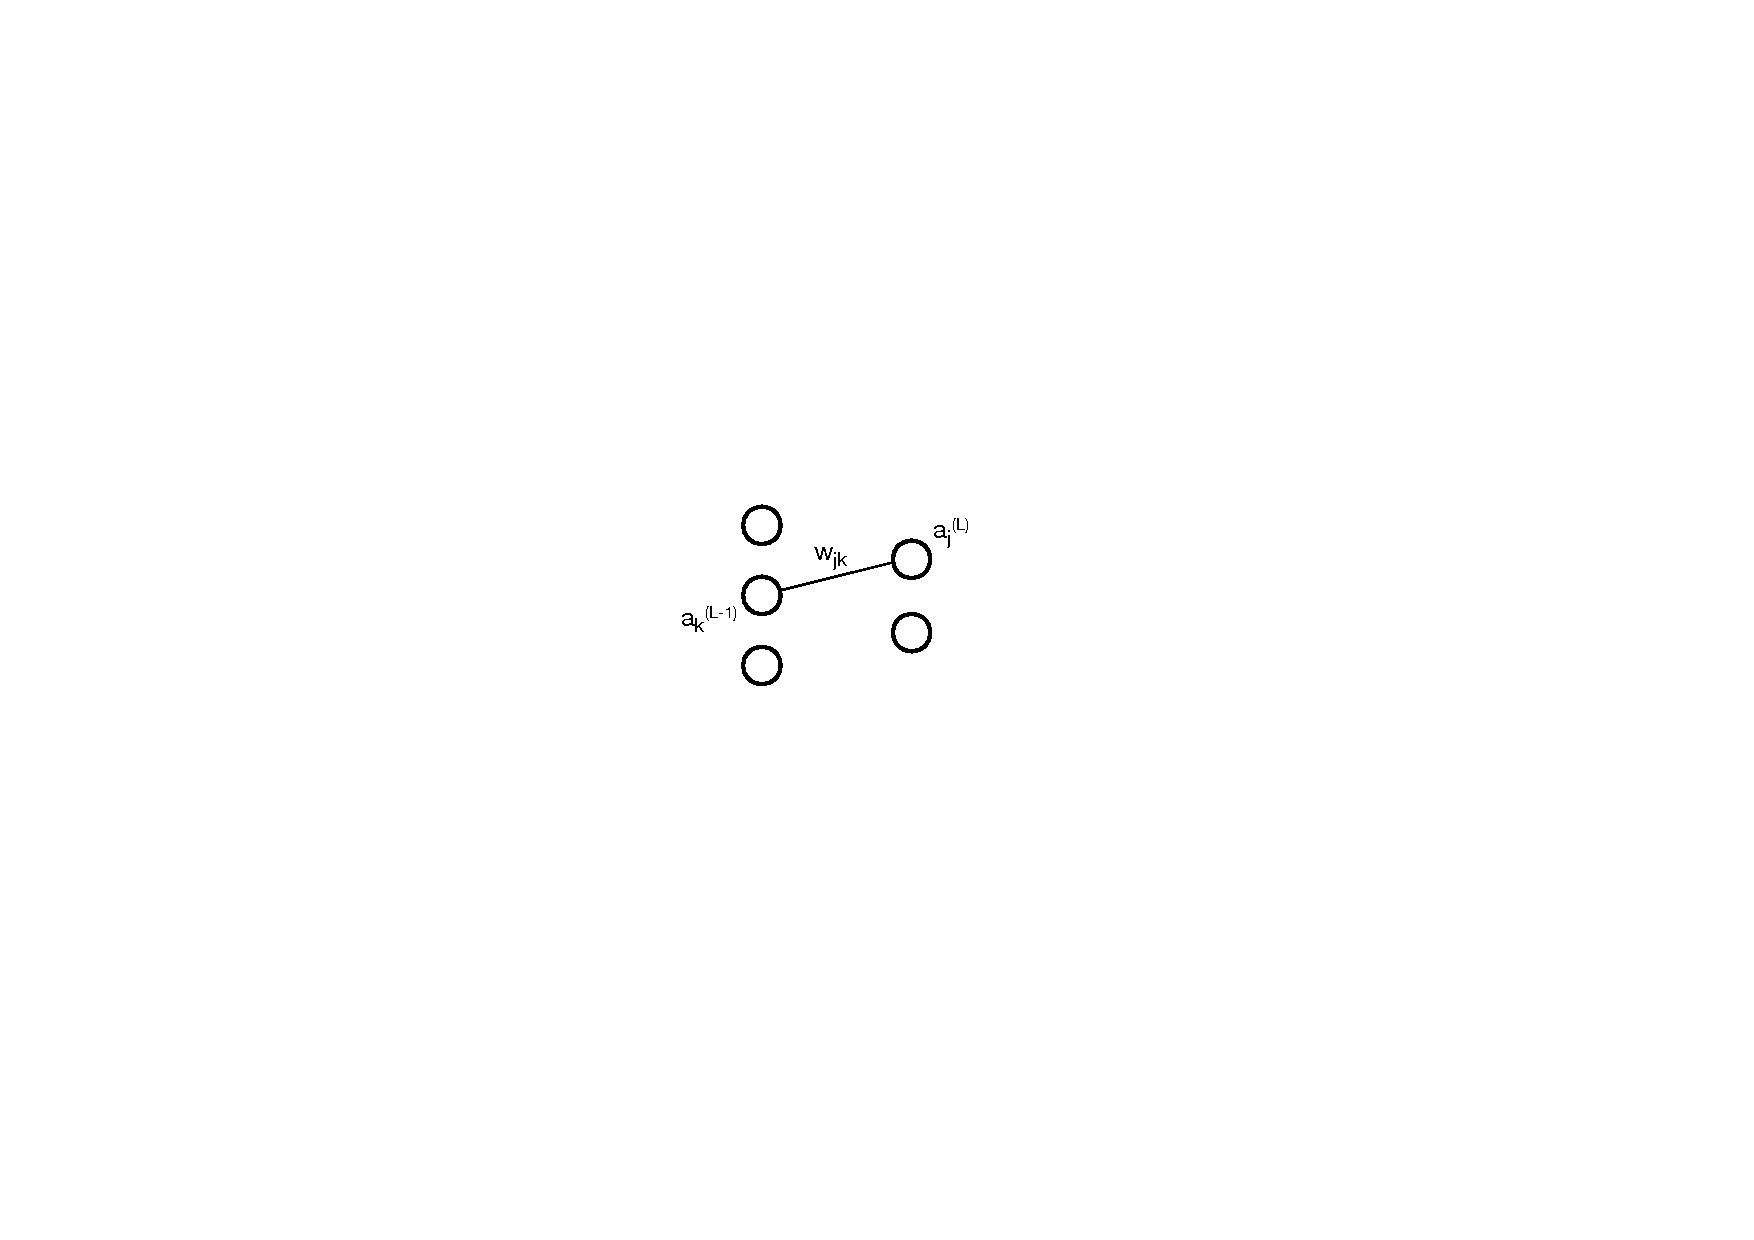
\includegraphics[width=0.3\linewidth]{figures/network-fragment.pdf}
}
\caption{A fragment of a neural network exposing the relation between activation of the $k$-th neuron in layer $(L-1)$ and activation of a $j$-th neuron at leyer $L$.}
\label{fig:network-fragment}
\end{figure}

Let us consider now a more general type of network, with a number of neurons at each layer, and the number of neurons at the output layer. We again restrict the training set to only one data instance. Consider a fragment of a network from Fig.~\ref{fig:network-fragment}, which depicts the relation between activation of the $k$-th neuron in layer $(L-1)$ and $j$-th neuron at leyer $L$. Notice that
\begin{align}
z_j^{(L)} & = \sum_i w_{ji}^{(L)} a_i^{(L-1)} + b_j^{(L)}, \\
a_j^{(L)} & = \sigma(z_j^{(L)}), \\
J & = \sum_j^(n_{L-1}(a_j^{(L)}-y_j)^2.
\end{align}
We assume the indices run from 0, replace the intercepts $b$ for each $k$-th neuron with $w_{0k}$, and denote the number of neurons at layer $L$ with $n_L$. Notice also that the weights have now two indices. The weight $w_{jk}$ is a weight for a $j$-the neuron for the output of the $k$-th neuron from the previous layer. For a gradient descent, we again need to compute the change this weight invokes to the cost function,
\begin{equation}
\pd{J}{w_{jk}}=\sum_j\pd{z_j^{(L)}}{w_{jk}} \times \pd{a_j^{(L)}}{z_j^{(L)}} \times \pd{J}{a_j^{(L)}}
\end{equation}
The partial derivatives of the first two terms in the product are straightforward, and stem directly from the expression for $z_j^{(L)}$ and $a_j^{(L)}$. But the partial derivative in the last term is new, and we can break it down to
\begin{equation}
\pd{J}{a_k^{(L-1)}} = \sum_{j=0}^{n_L} \pd{z^{(L)}}{a_k^{(L-1)}} \times \pd{a_j^{(L)}}{z_j^{(L)}} \times \pd{J}{a_j^{(L)}}
\end{equation}
With these two expressions, we can now chain back through the network and compute the influence of every of the network's parameters, thus providing means for the gradient descent. The procedure is known under the name {\em back propagation}, which, intuitively:
\begin{itemize}
	\item converts discrepancy between output and and target into error derivative,
	\item computes the error derivatives in each hidden layer from error derivatives of the next layer,
	\item uses error derivative with respect to activations to get error derivative with respect to weights.
\end{itemize}

Let us express our derivations and back-propagation procedure in a matrix form. We will assume that the input data includes $m$ data instances and $n$ features, and will for convenience add a first column of $1$'s to the input data matrix, thus increasing its size to $m\times (n+1)$ and denoting this matrix with $\X'$. Let this matrix represent the activations of the neurons in the first, input layer:
\begin{equation}
\A^{(1)}=\X'
\end{equation}
Then we can write the equations for the second layer:
\begin{align}
\underset{m\times n_2}{\Z^{(2)}} & = \underset{m\times n_1}{\A}^{(1)} \underset{n_1\times n_2}{\W}^{(2)} \\
\underset{m\times n_2}{\A^{(2)}} & = \sigma\left( \underset{m\times n_2}{\Z^{(2)}} \right)
\end{align}
For the general $l$-th layer we can write:
\begin{equation}
A^{(l)} = \sigma\left(A^{(l-1)} W^{(l)}\right)
\end{equation}

We start with the last layer,
\begin{equation}
\pd{J}{\W^{(L)}} = \pd{\Z^{(L)}}{\W^{(l)}} \times \pd{\A^{(L)}}{\Z^{(L)}} \times \pd{J}{\A^{(L)}}
\end{equation}
where computing the first partial derivative is straightforward. Let us represent the product of the last two terms with $\mathrm{d}$:
\begin{align}
\underset{m\times n_L}{\mathrm{d}^{(L)}} & = \left(\A^{(L)}-\Y \right)  \odot \A^{(L)} \left( 1-\A^{(L)}\right) \\
\pd{J}{\W^{(L)}} & = {1\over m} \left(\A^{(L-1)} \right)^\tr \times \mathrm{d}^{(L)}
\end{align}
where with $\odot$ we denote element-wise product. In a similar way we compute the partial derivative $\pd{J}{\A^{(L-1)}}$ as a function of partial derivate of $\pd{J}{\A^{(L)}}$, and repeat the computation of the above two equations for lower levels of the network.

\section{Bag of tricks}

As with training of other classifiers and regression models, like linear and logistic regression, there are technique which can speed up and improve convergence of the training of neural networks. These, in brief, include:
\begin{itemize}
	\item To aim to prevent overfitting, we can use regularization, and include the sum of all the weights of the network in a cost function. This procedure was also known as a {\em weight decay}, where after the computation of each weight these well further scaled down by some factor, say $0.99$. Notice that if using sigmoid activation function, the small weights meant that we operate at the linear part of sigmoid at thus with regularization aim at derive close-to-linear model, thus simplifying it.
	\item Neural networks include many parameters, the problem we can alleviate through {\em weight sharing}. That is, neurons at some level would share some of the weights.
	\item Training of neural networks assumes large training data set. We can use all of the data instances from the training data, but for large data sets use {\em mini-batch} gradient descent with adaptive learning rate and use of momentum in the optimization.
	\item To further avoid overfitting, we can use {\em dropout}, where we randomly drop neurons along with their connections from the neural network during the training. Dropout prevents neurons from co-adapting. During training, dropout samples form an exponential number of different ``thinned'' networks, thus also, in some way, introduce ensembling.
\end{itemize}

These and other tricks and their details go beyond our discussion in this chapter. They are all implemented in today standard packages for neural network training. While one of the homeworks of this course will be on neural network implementation, this, and the derivation of related equations and their implementation would almost certainly be a once-in-a-lifetime attempt useful only for educational reasons.

\printbibliography[heading=subbibliography]
\end{refsection}


\end{document}
